\documentclass[12pt,
a4paper
]{report}

%Dados que precisam ser customizados em todo projeto. Ex.: Titulo, Autor, Orientador, etc 
\makeatletter
%Declaração das variáveis
\newcommand{\nomeuniversidade}[1]{\gdef\@nomeuniversidade{#1}}
\newcommand{\nomeinstituto}[1]{\gdef\@nomeinstituto{#1}}
\newcommand{\nomeinstitutoparceiro}[1]{\gdef\@nomeinstitutoparceiro{#1}}
\newcommand{\nomeprograma}[1]{\gdef\@nomeprograma{#1}}
\newcommand{\siglaprograma}[1]{\gdef\@siglaprograma{#1}}
\newcommand{\subtitulo}[1]{\gdef\@subtitulo{#1}}
\newcommand{\cidade}[1]{\gdef\@cidade{#1}}
\newcommand{\orientador}[1]{\gdef\@orientador{#1}}
\newcommand{\coorientador}[1]{\gdef\@coorientador{#1}}
\newcommand{\orientadorestitulo}[1]{\gdef\@orientadorestitulo{#1}}
\newcommand{\textofolharosto}[1]{\gdef\@textofolharosto{#1}}
\newcommand{\siglauniversidade}[1]{\gdef\@siglauniversidade{#1}}


%Local onde devem ser alteradas as informações gerais do trabalho
\nomeuniversidade{Universidade Federal do Rio de Janeiro}
\nomeinstituto{Instituto de Computação}
\nomeinstitutoparceiro{Instituto Tércio Pacitti de Aplicações e Pesquisas Computacionais}
\nomeprograma{Programa de Pós-Graduação em Informática}
\siglaprograma{PPGI}
\author{Nome do(a) Autor(a) do Trabalho}
\title{Título do Trabalho}
%Caso o trabalho não tenha subtítulo, basta deixar o conteudo do comando subtitulo em branco.
% Ex:\subtitulo{}
\subtitulo{: subtítulo do trabalho}
\cidade{Rio de Janeiro}
\date{2026}

\orientador{Nome do(a) Orientador(a)}
\coorientador{Nome do(a) Co-orientador(a)}
\orientadorestitulo{D.SC}
\textofolharosto{Dissertação de Mestrado apresentada ao \@nomeprograma, \@nomeinstituto\ e  \@nomeinstitutoparceiro, \@nomeuniversidade, como requisito parcial à obtenção do título de Mestre em Informática.}
\siglauniversidade{UFRJ}


\makeatother

%Configurações gerais do projeto, como pacotes e suas configurações específicas. 
%Normalmente não precisam ser alterados
%Configuração do idioma usado no documento
\usepackage[brazilian]{babel}

%Definição padrao das margens das paginas
\usepackage[top=3cm,                    
bottom=2cm,
left=3cm,
right=2cm]{geometry}

%%%%% Configuração do espacamento padrão do documento - INICIO  %%%%%%%%%%%%%%%%%%%%%%%%
\usepackage{setspace}  % pacote usado para define o espacamento entre linhas do texto e de partes especificas
\onehalfspacing % definindo espaçamento padrao de 1,5 nas entrelinhas
%%%%% Configuração do espacamento padrão do documento - FIM  %%%%%%%%%%%%%%%%%%%%%%%%

% Usado para melhorias de alinhamento e justificação do texto
\usepackage{microtype}

% Usado Para permitir utilizar nomes de cores em diversos pacotes
\usepackage[table]{xcolor}

% Usado Para identar também intentar a primeira linha do primeiro parágrafo das subseções
\usepackage{indentfirst}

% Pacote da fonte escolhida: Opções de fontes em: https://ctan.org/topic/font
\usepackage{opensans}                    


%%%%% Removendo da contagem a capa e a ficha catalográfica - INICIO  %%%%%%%%%%%%%%%%%%%%%%%%
\addtocounter{page}{-2} 
%%%%% Removendo da contagem a capa e a ficha catalográfica - FIM  %%%%%%%%%%%%%%%%%%%%%%%%

% Usado nas referencias de equações, através do comando \eqref
\usepackage{amsmath}

% Necessario para incluir a ficha catalográfica, anexos e apêndices
\usepackage{pdfpages} 


% Usado para remover a quebra de linha nos recuos das folhas de rosto e de aprovação
\usepackage{hyphenat}                   

% Usado para justificar o texto nos recuos das folhas de rosto e de eprovação
\usepackage{ragged2e}                   

%%%%% Pacote e configurações da paginação - INICIO %%%%%%%%%%%%%%%%%%%%%%%%
\setlength{\headheight}{15.3pt} %Corrige warning do header do pacote fancyhdr
\usepackage{fancyhdr} % Pacote utilizado para alterar a posicao da paginação

%Redefine o style plain
\pagestyle{fancy}
\fancyhf{} % Limpa todos os cabeçalhos e rodapés padrão
\fancyhead[R]{\thepage} % Coloca o número da página no canto superior direito
\renewcommand{\headrulewidth}{0pt} % Remove a linha do cabeçalho (opcional)
\fancypagestyle{plain}{
	\fancyhf{} % Limpa cabeçalhos e rodapés
	\fancyhead[R]{\thepage} % Número da página no canto superior direito
	\renewcommand{\headrulewidth}{0pt} % Remove a linha do cabeçalho
}
%%%%% Pacote e configurações da paginação - INICIO %%%%%%%%%%%%%%%%%%%%%%%%



%%%%% Configurações de links das referencias internas e externos - INICIO  %%%%%%%%%%%%%%%%%%%%%%%%
\usepackage{hyperref} % Cria os links das referencias internas e para links externos tb
\makeatletter
\hypersetup{
	pdftitle={\@title},
	pdfpagemode=FullScreen,
	colorlinks=true,      % Ativa a coloração dos links
	linkcolor=black,     % Cor dos links internos
	citecolor=black,     % Cor das citações
	urlcolor=black       % Cor dos links de URL
}
\makeatother
%%%%% Configurações de links das referencias internas e externos - FIM  %%%%%%%%%%%%%%%%%%%%%%%%



%%%%% Configuração do estilo CSL usado na bibilografia - INICIO %%%%%%%%%%%%%%%%%%%%%%%%%%%%%%%%
\usepackage[style=config/template-ibict-completo-20251112]{citation-style-language}
\addbibresource{3-pos-textuais/referencias.bib}
%%%%% Configuração do estilo CSL usado na bibilografia - FIM %%%%%%%%%%%%%%%%%%%%%%%%%%%%%%%%%%%


%%%%% Configurações do texto de Fonte das imagens - INICIO  %%%%%%%%%%%%%%%%%%%%%%%%
\usepackage{copyrightbox} % Necessario para adicionar origem das imagem e das tabelas
\makeatletter
\renewcommand{\CRB@setcopyrightfont}{%
	\color{black}
}
\makeatother
%%%%% Configurações do texto de Fonte das imagens - FIM  %%%%%%%%%%%%%%%%%%%%%%%%



%%%%% Evita reiniciar numeracoes das equações nos capitulos - INICIO  %%%%%%%%%%%%%%%%%%%%%%%%
\usepackage{chngcntr} % Permite modificar a numeração dos contadores: Equacoes, Tabelas, e Figuras
\counterwithout{equation}{chapter} % Remove a reinicialização da numeração a cada capítulo
% A configuração de tabela e figura estão em  seus respectivos arquivos de listagem 
% juntamente com as suas demais configurações 
%%%%% Evita reiniciar numeracoes das equações nos capitulos - FIM  %%%%%%%%%%%%%%%%%%%%%%%%


%%%%% Pacote que permite criar indices - INICIO  %%%%%%%%%%%%%%%%%%%%%%%%
\usepackage{imakeidx} % Pacote para criar o índice
\makeindex[columns=3, options= -s config/estilo-indice.ist] % Configura quantidade de colunas do índice e o arquivo de estilo
%%%%% Pacote que permite criar indices - FIM  %%%%%%%%%%%%%%%%%%%%%%%%


% Permite alterar o formato das listas enumeradas 
\usepackage{enumitem}                   

%\usepackage{url}                        % Usado para formatar URLs no texto





%%%%% Formatação da lista de figura e de tabelas - INICIO  %%%%%%%%%%%%%%%%%%%%%%%%
\usepackage{titletoc} % Pacote para formatar sumário, lista de figuras e tabelas

%a configuração só funciona se for antes do documentclass

%Lista de Tabelas
\titlecontents{figure}[0pt]
{}
{\figurename\ \thecontentslabel\ - }
{}
{\titlerule*[0.4pc]{.}\contentspage}
[\addvspace{5pt}]

%Lista de Tabelas
\titlecontents{table}[0pt]
{}
{\tablename\ \thecontentslabel\ - }
{ }
{\titlerule*[0.4pc]{.}\contentspage}
[\addvspace{5pt}]
%%%%% Formatação da lista de figura e de tabelas - FIM  %%%%%%%%%%%%%%%%%%%%%%%%



%%%%% Formatação dos titulos dos capitulos, secao, subsecao, etc - INICIO  %%%%%%%%%%%%%%%%%%%%%%%%
\usepackage{titlesec}

\titlespacing{\chapter}
  {0pt}   % Espaço à esquerda
  {-17pt}   % Espaço acima do título do capítulo (é aqui que se reduz)
  {15pt}  % Espaço abaixo do título do capítulo

\titleformat{\chapter}[hang] % shape
{\normalsize\bfseries\uppercase} % format
{\thechapter}
{10pt}
{}

\titleformat{\section}[hang] % shape
{\normalsize\normalfont\uppercase} % format
{\thesection}
{10pt}
{}

\titleformat{\subsection}[hang] % shape
{\normalsize\bfseries} % format
{\thesubsection}
{10pt}
{}

\titleformat{\subsubsection}[hang] % shape
{\normalfont\normalsize} % format
{\thesubsubsection}
{10pt}
{}

\titleformat{\paragraph}[hang] % shape
{\normalfont\normalsize} % format
{\theparagraph}
{10pt}
{}

\titleformat{\subparagraph}[hang] % shape
{\normalfont\normalsize} % format
{\thesubparagraph}
{}
{}
%%%%% Formatação dos titulos dos capitulos, secao, subsecao, etc - FIM  %%%%%%%%%%%%%%%%%%%%%%%%

% pacote que gera textos aletorios, pode remover quando for realizar o trabalho
\usepackage{lipsum} 




%%%%% Definindo melhor configuração das imagens - INICIO %%%%%%%%%%%%%%%%%%%%%%%%
\usepackage{float}
%%%%% Definindo melhor configuração das imagens - FIM %%%%%%%%%%%%%%%%%%%%%%%%



%%%%% Definindo diretorios padrao do template e do projeto - INICIO %%%%%%%%%%%%%%%%%%%%%%%%
\usepackage{graphicx}		            % Inclusão de gráficos, pdfs
\graphicspath{{figuras/}{figuras/modelo}}
%%%%% Definindo diretorios padrao do template e do projeto - INICIO %%%%%%%%%%%%%%%%%%%%%%%%

%inicio do documento
\begin{document}

	%%%%%%%%%%%%%%%%%%%%%%%%%%%%%%%%%%
	%  Elementos pré textuais
	%%%%%%%%%%%%%%%%%%%%%%%%%%%%%%%%%%
	%Capa do documento (elemento obrigatório)
	%Remove a paginação desse documento
\thispagestyle{empty}

%Habilita o uso de variáveis
\makeatletter

\begin{center}
	
	%Adiciona as imagens dda universidade e do programa/instituto
	\noindent
	
\includegraphics{logo_ufrj_capa.pdf}%
	\hfill
	
\includegraphics{logo_programa_capa.pdf}
	\vspace{1cm}
	
	% As variáveis @nomeuniversidade, @nomeinstituto, @nomeinstitutoparceiro, @author, @title, @subtitulo, @cidade e @date dessa página,
	% podem ser ajustadas no arquivo config/informacoes_gerais.tex
	\MakeUppercase{\@nomeuniversidade}\\
	\MakeUppercase{\@nomeinstituto}\\

	%%%%%%%%%%%%%%%%%%%%%%%%%%%%%%%%%%%%%%%%%%%%%%%%%%%%
	% Configuração mestrado/doutorado e graduação
	%%%%%%%%%%%%%%%%%%%%%%%%%%%%%%%%%%%%%%%%%%%%%%%%%%%%
	% Para mestrado e doutorado: descomentar as variáveis desse bloco e comentar a do próximo bloco
	\MakeUppercase{\@nomeinstitutoparceiro}\\
	\MakeUppercase{\@nomeprograma} (\@siglaprograma)
	%%%%%%%%%%%%%%%%%%%%%%%%%%%%%%%%%%%%%%%%
	% Para tcc: Descomentar a variável desse bloco e comentar as do bloco de cima
	%\MakeUppercase{\@nomecursograduacao}\\
	%%%%%%%%%%%%%%%%%%%%%%%%%%%%%%%%%%%%%%%%
	
	\vspace{2cm}
	\textbf{\MakeUppercase{\@author}}
	
	\vspace{4cm}
	\MakeUppercase{\@title}\@subtitulo
	
	\vspace*{\fill}
	\MakeUppercase{\@cidade}\\
	\@date
	
\end{center}
\makeatother

	%Folha de rosto do documento (elemento obrigatório)
	\thispagestyle{empty}
\makeatletter
\begin{spacing}{1}
\begin{center}

% As variáveis @faculdade, @instcomp, @instnce, @programa, @progsigla,
% @author, @title, @subtitulo, @textofolharosto, @orientadora,
% @coorientadora, @orientadorastitulo, @cidade, e @date dessa página
% podem ser ajustadas no arquivo config/informacoes_gerais.tex
\large \MakeUppercase{\@nomeuniversidade}

\large \MakeUppercase{\@nomeinstituto}

\large \MakeUppercase{\@nomeinstitutoparceiro}

\large \MakeUppercase{\@nomeprograma} (\@siglaprograma)

\vspace{2cm}
\large \MakeUppercase{\@author}

\vspace{2cm}
\large \textbf{\MakeUppercase{\@title}\@subtitulo}
\end{center}

\vspace{0.5cm}
\epigraph{\normalsize\justifying\nohyphens{\@textofolharosto}}

\vspace{2cm}
Orientadora: Profa. \@orientador, \@orientadorestitulo

Co-orientadora: Profa. \@coorientador, \@orientadorestitulo

\vspace*{\fill}
\begin{center}
\@cidade\\
\@date
\end{center}

\end{spacing}
\makeatother
\newpage

	%Ficha catalográfica do documento (elemento obrigatório)
	\input{1-pre-textuais/ficha_catalografica}

	%Folha de aprovação do documento (elemento obrigatório)
	\thispagestyle{empty}
\makeatletter
\begin{spacing}{1}
\begin{center}

% As variáveis @author, @title, @subtitulo, @textofolharosto,
% @orientadora, @coorientadora, @orientadorastitulo,
% @progsigla, @faculdadesigla e  dessa página
% podem ser ajustadas no arquivo config/informacoes_gerais.tex
\large \MakeUppercase{\@author}

\vspace{1.5cm}
\large \textbf{\MakeUppercase{\@title}\@subtitulo}

\end{center}

\vspace{0.5cm}
\epigraph{\normalsize\justifying\nohyphens{\@textofolharosto}}

\vspace{1.5cm}
Aprovado em 30 de março de \@date\ por:

\vspace{2cm}
\begin{flushright}

\hspace{5cm} \hrulefill

Prof(a). \@orientador, \@orientadorestitulo, \@siglaprograma/\@siglauniversidade (Presidente)

\vspace{2cm}
\hspace{5cm} \hrulefill

Prof(a). \@coorientador, \@orientadorestitulo, \@siglaprograma/\@siglauniversidade

\vspace{2cm}
\hspace{5cm} \hrulefill

Prof(a). Nome do Representante da Banca, \@orientadorestitulo, NCE/\@siglauniversidade


\vspace{2cm}
\hspace{5cm} \hrulefill

Prof(a). Nome do Representante da Banca, \@orientadorestitulo, \@siglaprograma/\@siglauniversidade

\end{flushright}

\end{spacing}
\makeatother
\newpage

	%Dedicatória do documento (elemento opcional)
	\newpage
\thispagestyle{empty}
\begin{spacing}{1}
	\vspace*{\fill}

	\noindent
	\hfill\parbox{9cm}{Dedico esse trabalho aos meus pais, por todo amor, dedicação e compreensão. Amo vocês.}

\end{spacing}


	%Agradecimento do documento (elemento opicional)
	\newpage
\thispagestyle{empty}
\begin{center}
\textbf{\MakeUppercase{Agradecimentos}}
\end{center}


\lipsum[1-4]

	%Epígrafe do documento (elemento opicional)
	\newpage
\thispagestyle{empty}
\begin{spacing}{1}
	\vspace*{\fill}

	\noindent\hfill\parbox{9cm}{
		\textit{``Descrever o texto da citacao utilizada na epígrafe desse template de trabalho.\\
			O texto pode ter mais de uma linha caso se deseje.\\
			Ou pode ser em um texto longo também. de acordo com a necessidade e com a escolha feita.''}
	}\\[2ex]
	\hspace*{\fill}(Nome do Autor)

\end{spacing}





	%Resumo do documento (elemento obrigatório)
	\newpage
\thispagestyle{empty}
\begin{center}
	\textbf{\MakeUppercase{Resumo}}
\end{center}

\noindent
Utilize, de preferência, um só parágrafo para descrever os objetivos de seu trabalho acadêmico, o método com informações sobre coleta, tratamento e análise dos dados, as técnicas de abordagem, os resultados e suas principais conclusões. Esse resumo deve conter de 150 a 500 palavras. Deve ser evitado o uso de frases negativas, símbolos ou contrações que não sejam de uso corrente, fórmulas, equações, diagramas etc. que não sejam absolutamente
necessários; quando for indispensável, defini-los na primeira vez que aparecerem. Texto adaptado do Manual do Sibi da UFRJ diponível em \cite{ManualSibi2025}.

\vspace{1em}
\noindent
Palavras-chave: palavras; chave; separadas; por; ponto e vírgula

	%Abstract do documento (elemento obrigatório)
	\newpage
\thispagestyle{empty}
\begin{center}
	\textbf{\MakeUppercase{Abstract}}
\end{center}

\noindent
Traduza seu resumo para o idioma de
divulgação internacional escolhido por você e seu orientador. Traduza também as palavras-chave.

\vspace{1em}
\noindent
Keywords: key; words; separated; by; semi commas

	%Lista de figuras do documento (elemento optional, mas fortemente recomendado)
	\input{1-pre-textuais/lista_figuras}

	%Lista de tabelas do documento (elemento optional, mas fortemente recomendado)
	\input{1-pre-textuais/lista_tabelas}

	%Lista de siglas do documento (elemento optional, mas fortemente recomendado)
	\newpage
\thispagestyle{empty}
\begin{center}
\textbf{\uppercase{Lista de Abreviaturas e Siglas}}
\end{center}
\vspace{0.5cm}

\begin{spacing}{2}

\begin{longtable}[l]{ l l }
\hypertarget{sigla:AI}{\textbf{AI}}&Artificial Intelligence\\
\hypertarget{sigla:CPU}{\textbf{CPU}}&Central Process Unit\\
\hypertarget{sigla:FSP}{\textbf{FSP}}&Feature Space Partition\\
\hypertarget{sigla:GPU}{\textbf{GPU}}&Graphical Process Unit\\
\hypertarget{sigla:IA}{\textbf{IA}}&Inteligencia Artificial\\
\hypertarget{sigla:KNN}{\textbf{K-NN}}&K-Nearest Neighbors\\
\hypertarget{sigla:ML}{\textbf{ML}}&Machine Learning\\
\hypertarget{sigla:PyPI}{\textbf{PyPI}}&Python Package Index\\
\hypertarget{sigla:SVM}{\textbf{SVM}}&Support Vector Machine
\end{longtable}
{\addtocounter{table}{-1}}

\end{spacing}


	%Sumário do documento (elemento obrigatório)
	\addtocontents{toc}{\protect\thispagestyle{empty}} % força o "empty" na primeira pagina do sumário
\pagestyle{empty} % remove a numeracao das demais paginas de sumario (se houver mais de uma) 

%apresenta ate o nivel 5, de paragrafo
\setcounter{tocdepth}{4}

%apresenta a numeracao ate o nivel 5, de paragrafo
\setcounter{secnumdepth}{4}

% A definição desse comando que estabelece qual o ponto de início do texto (ou seja a margem do texto) dos ítens do sumário.
% Ajuste o valor do espaçamento para a que representa o nível de maior profundidade do seu trabalho
% Por exemplo, se o seu trabalho possui uma subsecao de nível x.x.x (ex 1.2.3), deixe descomentado apenas a configuração de terceiro nível, de valor 32pt. O padrão desse documento são dois níveis (valor 23pt)
% 1 - nível: \newcommand{\sumariotextmarginlenght}{13pt}
% 2 - nível: \newcommand{\sumariotextmarginlenght}{23pt}
% 3 - nível: \newcommand{\sumariotextmarginlenght}{32pt}
% 4 - nível: \newcommand{\sumariotextmarginlenght}{38pt}
% 5 - níveil: \newcommand{\sumariotextmarginlenght}{46pt}
\newcommand{\sumariotextmarginlenght}{23pt}

% titletoc - Configuração da formatação dos títulos (em seus vários níveis) no sumário. 
% A formatação desses mesmos títulos dentro do texto, precisa ser feito antes do begin{document} e ficou no arquivo: config/configuracoes.tex
\titlecontents{chapter}[\sumariotextmarginlenght]
{\normalfont\normalsize\bfseries}
{\contentslabel{\sumariotextmarginlenght}\uppercase} % removido \MakeUppercase
{}
{\titlerule*[0.4pc]{.}\contentspage} % aqui sim!

\titlecontents{section}[\sumariotextmarginlenght]
{\normalfont\normalsize}
{\contentslabel{\sumariotextmarginlenght}\uppercase}
{}
{\titlerule*[0.4pc]{.}\contentspage}

\titlecontents{subsection}[\sumariotextmarginlenght]
{\normalfont\normalsize\bfseries}
{\contentslabel{\sumariotextmarginlenght}}
{}
{\titlerule*[0.4pc]{.}\contentspage}

\titlecontents{subsubsection}[\sumariotextmarginlenght]
{\normalfont\normalsize}
{\contentslabel{\sumariotextmarginlenght}}
{}
{\titlerule*[0.4pc]{.}\contentspage}

\titlecontents{paragraph}[\sumariotextmarginlenght]
{\normalfont\normalsize}
{\contentslabel{\sumariotextmarginlenght}}
{}
{\titlerule*[0.4pc]{.}\contentspage}


%Altera e Formata o titulo do sumario
\renewcommand{\contentsname}{\normalsize\centerline{\bfseries\uppercase{Sumário}}}

\tableofcontents % Insere o sumário
\clearpage % Garante que o sumário termine aqui
\pagestyle{fancy} % Retorna ao estilo "fancy" para o restante do documents

	%%%%%%%%%%%%%%%%%%%%%%%%%%%%%%%%%%
	%  Elementos principais do texto
	%%%%%%%%%%%%%%%%%%%%%%%%%%%%%%%%%%
	%Introdução do documento (elemento obrigatório)
	\chapter{Introdução}

Antes de abordar os tópicos que são objetivos deste guia, é importante estabelecer alguns pontes que devem ser levados em consideração, durante a criação do seu trabalho:

\begin{enumerate}
	\item Esse guia não é uma norma, é uma sugestão. Não tem como objetivo engessar a escrita. É uma sugestão de encadeamento dos itens inerentes ao processo de pesquisa, utilizando a formatação indicada pelo SiBI.
	\item Mais importante que o guia em si, é formar um pesquisador e deixar brotar seu estilo autoral a partir da convivência científica com seu orientador.  A elaboração do texto virá da interação orientador e orientando e deverá respeitar o estilo da comunidade acadêmica a que pertence.
	\item Esse documento foi elaborado dentre outras coisas a partir das diretivas do (SIBI UFRJ, 2025) e de (Silva, 2006) [Silva, 2025 - notas de aula da disciplina Metodologia de Pesquisa Científica ofertada em cursos lato e stricto sensu da UFRJ.]
	\item Esse guia não substitui a leitura e uso do Manual de formatação do SiBI.
	\item Esta versão do guia já está alinhada com a 9ª revisão do manual do SiBI \cite{ManualSibi2025}, de agosto de 2025.
	\item Caso esse material tenha sido útil tanto para a formatação quanto para o entendimento do que se espera de um trabalho acadêmico, e caso deseje, ficamos agradecidos com uma possível citação do nosso trabalho. Esse guia está contido dentro do que foi denominado Projeto Jacurutu \cite{Projeto_Jacurutu} e pode ser citado da mesma forma que a citação anterior e  cuja referência está presente na seção de Referências desse guia.
\end{enumerate}

Agora voltando ao objetivo desse guia, a seção introdutória versa sobre a apresentação inicial do trabalho acadêmico e deve indicar a motivação ou problemática, os objetivos da pesquisa, a relevância, a delimitação do assunto tratado e outros elementos necessários para situar o leitor.

Seja sucinto para não cansar o leitor, pois na introdução ele quer apenas uma ideia inicial do que virá à frente. Contudo, não deixe de “vender” a ideia, a relevância e as contribuições que emergirão do seu trabalho acadêmico nas próximas seções.

\section{Motivação ou problemática}

Relatar o que motivou a executar essa pesquisa, seja uma motivação da sua experiência pessoal ou uma motivação com base em problemas sociais atuais.

\section{Objetivos da pesquisa}

Nesta parte, você deve salientar qual o fenômeno a ser investigado e quais os objetivos principais e secundários ao pesquisar esse fenômeno.

Esta monografia visa responder qual pergunta? É importante que o aluno deixe claro a pergunta da pesquisa.

O objetivo pode ser organizado em Objetivo Geral e Objetivos Específicos, caso você queira falar do objetivo final e das partes que você precisará fazer para atingi-lo. Ou pode ser organizado em Objetivo Primário e Objetivos secundários, onde você fala do seu objetivo principal e de outros que você alcançará após a realização do primeiro.

\section{Relevância}

Por que é importante estudar esse tema? Qual a relevância acadêmica e prática de investigar tal assunto? 

A relevância fica diminuída quando apenas o próprio autor da monografia parece considerá-la importante. Assim, preferencialmente, a relevância deve ser levantada a partir da leitura de outros autores. Cite outros autores que consideram importante o estudo de tal tema.

\section{Delimitação da pesquisa}

A seção de delimitação de estudo visa demarcar o escopo de sua pesquisa, indicando ao leitor partes que não serão o alvo da sua investigação.

\section{Estrutura do trabalho}

O restante deste texto está organizado da seguinte forma. A Seção~\ref{cap:referencial_teorico} apresenta os conceitos básicos do referencial teórico necessário para um melhor entendimento do trabalho, com a apresentação dos assuntos tal, tal e tal. A Seção~\ref{cap:metodologia} relata qual foi a metodologia utilizada no trabalho. A Seção~\ref{cap:desenvolvimento} apresenta um detalhamento do  desenvolvimento do trabalho. Por fim a Seção~\ref{cap:conclusao} apresenta a conclusão, com um sumário dos resultados e sugestões para trabalhos futuros.

	%Referêncial Teórico do documento (elemento recomendado)
	\chapter{Referencial teórico}
\label{cap:referencial_teorico}

Faça uma compilação dos principais autores sobre o tema a ser investigado. Nesta fase é importante o apoio de seu orientador\index{orientador} e a clareza quanto ao tema e à pergunta da sua pesquisa, indicando o que é essencial ser lido e resumido e o que é secundário. A pergunta funciona como um guia do que deve ser exposto nessa seção e, principalmente, do que não é necessário.

A forma pela qual você estruturará esse seção já será uma de suas contribuições. Cada pesquisador, dentro de um mesmo tema, possui uma forma única de organizar o conhecimento compulsado.

O Referencial teórico\index{referencial teórico} é como uma aula sobre o tema para que o leitor consiga acompanhar as próximas seções de seu trabalho. Observe que não é um resumo de tudo que você aprendeu no seu curso.

Divida o assunto que você deseja estudar em seções. As seções devem conduzir o leitor pelos conceitos apresentados. Assim, você deve começar pelo tópico mais geral e ir especificando cada vez mais até trazer seu leitor ao tema específico de seu trabalho acadêmico. Dentro de cada seção, você pode usar subseções para organizar melhor a informação destacada.

\section{Assunto mais geral do referencial teórico} \label{sub:assunto2}

A primeira seção\index{seção} do referencial teórico normalmente será sobre o tema mais geral dentre os assuntos abordados no seu trabalho. 

\section{Assunto mais específico do referencial teórico}

As demais seções tendem a ser mais específicas que as anteriores

\section{Trabalhos relacionados}

Nessa seção, você pode elencar os trabalhos com os quais as suas contribuições podem ser comparadas na seção de discussão ao final do seu documento.
Para que o leitor\index{leitor} entenda as similaridades entre seu trabalho\index{trabalho} e os trabalhos correlatos, você deve, aqui, fazer um resumo de cada trabalho correlato realçando a interseção que eles possuem com os seus objetivos de pesquisa.

\section{Quadro referencial teórico}

Você pode incluir um quadro ao final do seu referencial destacando para o leitor quais foram as suposições ou hipóteses construídas a partir da literatura que você compilou. A palavra hipótese é mais utilizada em pesquisas quantitativas. A palavra suposição é mais utilizada em pesquisas mais interpretativas, qualitativas.

O trabalho \cite{DissertacaoElton2015}, por utilizar uma metodologia mista, apresenta exemplos de quadro de hipóteses e de quadro de suposições. A tabela~\ref{tab:quadro_hipoteses} apresenta uma parte do quadro de hipóteses\index{quadro de hipóteses} do trabalho.

\begin{table}[H]
	\caption{Exemplo de parte de um quadro de hipóteses.}
	\begin{center}
		\fontsize{10pt}{13pt}\selectfont
		\begin{tabular}{|p{0.1\linewidth}|p{0.4\linewidth}|p{0.4\linewidth}|}
			\hline
			\rowcolor{gray!10}
			\begin{center}
				\textbf{Hipótese}
			\end{center} &
			\begin{center}
				\textbf{Declaração}
			\end{center} &
			\begin{center}
				\textbf{Referencial}
			\end{center} \\
			\hline
			{\centering H1 \par} & O Prazer Percebido impacta da Utilidade Percebida. & Dias, 2001; Igbaria, Parasuraman e Baroudi, 1996. \\
			\hline
			{\centering H2 \par} & O Prazer Percebido impacta da Facilidade de Uso Percebida. & Dias, 2001; Igbaria, Parasuraman e Baroudi, 1996. \\
			\hline
			{\centering H3 \par} & O Prazer Percebido impacta na Intenção de Uso. & Dias, 2001; Igbaria, Parasuraman e Baroudi, 1996. \\
			\hline
			\multicolumn{3}{l}{Fonte: Adaptado de \cite[37]{DissertacaoElton2015}}
		\end{tabular}
		\label{tab:quadro_hipoteses}
	\end{center}
\end{table}

Ainda sobre o mesmo trabalho, a figura~\ref{tab:quadro_suposicoes} apresenta uma parte do quadro de suposições\index{quadro de suposições}.

\begin{table}[H]
	\caption{Exemplo de parte de um quadro de suposições.}
	\begin{center}
		\fontsize{10pt}{13pt}\selectfont
		\begin{tabular}{|p{0.1\linewidth}|p{0.4\linewidth}|p{0.4\linewidth}|}
			\hline
			\rowcolor{gray!10}
			\begin{center}
				\textbf{Hipótese}
			\end{center} &
			\begin{center}
				\textbf{Declaração}
			\end{center} &
			\begin{center}
				\textbf{Referencial}
			\end{center} \\
			\hline
			{\centering S1 \par} & Há uma tendência à utilização de celulares, smartphones e tablets como apoio a aprendizagem. & Santos, 2009; Mateus, Brito, 2011; Hoehle, Zhang, Venkatesh, 2015.. \\
			\hline
			{\centering S2 \par} & A presença de tutores presenciais no início do curso para ambientar os novos alunos é importante. & Mateus, Brito, 2011; Bizzaria et al. 2015.. \\
			\hline
			\multicolumn{3}{l}{Fonte: Adaptado de \cite[37]{DissertacaoElton2015}}
		\end{tabular}
		\label{tab:quadro_suposicoes}
	\end{center}
\end{table}


	%Metodologia do documento (elemento recomendado)
	\chapter{Metodologia de pesquisa}\label{cap:metodologia}

Essa seção existirá caso o estudante e seu orientador entendam que o conjunto de métodos de pesquisa utilizados no trabalho devem ser detalhados e relatados a fim de que o leitor acompanhe como a investigação científica foi desenvolvida. Essa seção apresenta os métodos de investigação utilizados, a ordem em que aparecem no texto e as razões para escolha de cada um deles, ou seja, qual o objetivo esperado com cada método.

Uma pesquisa pode fazer uso de um único método. E em alguns casos, orientador e estudante decidem colocar essa informação referente aos métodos de investigação em uma subseção da introdução.

A seção de metodologia difere da seção de resultados. A primeira aborda como os dados serão coletados e analisados, com qual método ou abordagem. A segunda relata os resultados advindos dessa coleta e dessa análise. Por exemplo, uma seção de análise demográfica dos dados deverá estar entre os resultados. 

São vários os métodos de pesquisa: estudo de caso, experimento, levantamento estatístico, fenomenologia, hermenêutica, etnografia, design science research, pesquisa-ação, ciência da implementação etc. O estudante deverá escolher os métodos que melhor se adequem ao tipo de contribuição que quer oferecer e que dialoguem com as pesquisas anteriores sobre o tema, permitindo que ele faça comparações com trabalhos correlatos. 

A Metodologia de Pesquisa pode ser dividida em subseções para melhor compreensão do leitor. Dependendo de cada método escolhido, poderá haver diferentes subseções. Segue uma sugestão que deverá se adequar ao estilo do estudante e de seu orientador.

\section{Tipo de pesquisa}
Quanto aos objetivos: sua pesquisa é exploratória, descritiva ou explicativa? Por quê?
Quanto aos meios: bibliográfica, documental, estudo de caso, etc... 

\section{Seleção dos sujeitos / Entrevistados}
Quantos são os entrevistados? Qual o cargo que ocupam e há quanto tempo? Por que é importante entrevistá-los?
Caso seja uma pesquisa mais objetiva: qual a população e a amostra? Qual a representatividade esperada?

\section{Coleta de dados}
Como será feita a coleta dos dados? A partir de documentação direta (observação do fenômeno ou entrevistas) ou indireta (leitura de dados sobre o fenômeno)? Se houver roteiro ou questionário, adicionar ao anexo.

\section{Análise de dados}
Como o pesquisador pretende fazer as análises dos dados que coletará? Usará alguma abordagem interpretativa caso a pesquisa seja qualitativa? Usará quais ferramentas de análise estatística caso esteja atuando com métodos quantitativos.

	%Desenvolvimento do documento (elemento obrigatório)
	\chapter{Desenvolvimento}\label{cap:desenvolvimento}

Como orientado pelo SIBI \cite{ManualSibi2025}, essa é a "parte principal do texto que contém a exposição ordenada e pormenorizada do assunto. Divide-se em seções e subseções, que variam em função da abordagem do tema e do método".

O texto referente ao desenvolvimento do trabalho versa sobre como o pesquisador executou o método de pesquisa. Assim, deverá descrever os dados coletados e analisá-los conforme o método prescreve. Alguns pesquisadores preferem descrever todos os dados e, em outra seção, analisá-los. Outros preferem descrever e analisar dado a dado.

\section{Construção de artefatos}
Caso o trabalho de pesquisa demande a construção de algum artefato (tecnológico ou teórico), sugerimos que seja feita uma seção específica para descrição do desenvolvimento desse artefato antes de usar os métodos de pesquisa que terão o objetivo de coletar e analisar os dados oriundos do uso desse artefato.

\section{Coleta de dados}
É o momento em que o pesquisador descreve para o leitor os dados que coletou. Seria como uma “foto” do fenômeno que o pesquisador observou. Não cabem críticas ou análises, apenas a exposição do que foi visto.

\section{Resultados da pesquisa}
No momento da análise dos dados, o pesquisador deve associar a teoria levantada no referencial teórico com os dados descritos anteriormente. Assim, o pesquisador realça se o que verificou na prática está de acordo, ou não, com a literatura.  O pesquisador pode e deve fazer comentários analíticos quanto ao que está diferente do que prega a teoria, realçando se tal diferença foi prejudicial, ou não.

É interessante salientar, também, o que está em consonância com o referencial teórico e verificar se essa concordância surtiu os efeitos benéficos citados pela teoria, ou não.

Essas análises feitas ao longo do desenvolvimento constituem os resultados da sua pesquisa. A seção de análise é comumente denominada "Resultados da pesquisa".

\section{Discussão dos resultados}
Após a apresentação dos resultados, o pesquisador pode criar uma seção de "Discussão dos resultados", em que confronta seus resultados com trabalhos correlatos, provavelmente citados na seção de referencial teórico.

\newpage
\textbf{Observações:} 
\begin{enumerate}
	\item As seções apresentadas anteriormente podem estar em um subnível dentro de uma seção maior chamada "Desenvolvimento", Como apresentado nesse guia; ou podem estar no mesmo nível da estrutura de seções que a Introdução, referencial e Metodologia;
	\item Caso o método utilizado fosse um experimento de um determinado aplicativo, antes da descrição dos dados coletados e de sua análise, haveria o relato do desenvolvimento do artefato que está sendo experimentado. Após isso, o pesquisador faria a descrição do ambiente pré-intervenção, a descrição da intervenção em si (incluindo configuração de ambiente necessária, softwares criados ou utilizados, etc) e a descrição pós-intervenção. A seguir, o autor poderia analisar as alterações percebidas com a intervenção à luz da teoria compulsada na seção de referencial teórico.
	\item Em um estudo de caso, o pesquisador poderia descrever caso a caso e depois analisá-los em busca de categorias que expliquem o fenômeno. Perceba que, dependendo do método de pesquisa utilizado, haverá diferenças na seção de desenvolvimento.
\end{enumerate}





	%Conslusão do documento (elemento obrigatório)
	\chapter{Conclusão}\label{cap:conclusao}

\section{Principais Contribuições}
Como orientado no Manual do SiBI, nessa seção o pesquisador retoma seus objetivos de pesquisa e suas hipóteses / suposições a fim de apresentar os principais resultados obtidos a partir da análise dos dados. Na seção anterior, o investigador fez uma análise minuciosa; aqui, resume os principais pontos, associando-os com os objetivos que pretendia alcançar. 

\section{Limitações da Pesquisa}
O pesquisador deve se antecipar e relatar os problemas encontrados na condução de sua pesquisa. Esse relato, além de mostrar o rigor metodológico e o compromisso com a busca da verdade, permite que o leitor entenda com mais clareza as decisões que nortearam a investigação.

\section{Pesquisas Futuras}\index{pesquisas futuras}
O pesquisador pode usar como inspiração para novas perguntas de pesquisa as limitações a que sua pesquisa esteve sujeita, ou seja, focar no que poderia ter sido feito de forma diferente para melhorar a coleta ou a análise dos dados. Ou qual outro método de pesquisa poderia ter sido utilizado e com quais objetivos.
Pode ainda, a partir dos resultados obtidos em sua investigação, propor novas questões acerca do fenômeno em estudo, estimulando a continuidade das pesquisas sobre o tema.

	%%%%%%%%%%%%%%%%%%%%%%%%%%%%%%%%%%
	%  Elementos pós textuais
	%%%%%%%%%%%%%%%%%%%%%%%%%%%%%%%%%%
	%Referencias do documento (elemento obrigatório)
	%Altera o nome da seção de bibliografia
\renewcommand{\bibname}{\normalsize\centerline{\bfseries\uppercase{Referências}}}

\phantomsection
\addcontentsline{toc}{chapter}{REFERÊNCIAS} % Adiciona a bibliografia ao índice
\begin{flushleft}
\begin{spacing}{1}
\printbibliography
\end{spacing}
\end{flushleft}

	%Glossário do documento (elemento opcional)
	\input{3-pos-textuais/glossario}

	%Exemplo de apêndice (desenvolvido pelo autor) (elemento opcional)
	\newpage
\phantomsection
\addcontentsline{toc}{chapter}{\MakeUppercase{Apêndice A - Informações técnicas e formatações}}
\begin{center}
\textbf{\MakeUppercase{Apêndice A - Informações técnicas e formatações}}
\end{center}

Os apêndices contidos nesse projeto, servem como exemplos que podem ser utilizados pelos autores que utilizam esse modelo. Lembrando que apêndices são complementos do trabalho que também foram produzidos pelo autor, conforme explicado no item 3.1.4.3 do Manual do SiBI \cite{ManualSibi2025}.

No Apêndice A, são apresentadas informações técinicas do modelo, como a explicação de alguns pacotes utilizados, e algumas funcionalidades do modelo bem como guns exemplos de itens e formatações que são corriqueiramente utilizadas em um documento {\LaTeX}, como Citações, Figuras, Tebelas e etc.

Maores informações técnicas sobre o modelo e os pacotes utilizados, podem ser obtidas na wiki do projeto \cite{wiki_jacurutu}.

O Apêndice B, apresenta um exemplo de um apêndice que foi incluído a partir de um outro documento do autor, mas no corpo do trabalho.

O Apêndice C é um exemplo de um formuário de pesquisa, produzido pelo próprio autor, mas que foi incluído com os comandos \LaTeX.

Seguem algumas informações técnicas sobre o modelo e alguns exemplos de itens mais comuns:

\begin{enumerate}
	\item \MakeUppercase{Citações}

	O conjunto de configurações estabelecidas pelo projeto Jacurutu, garatem que todas as citações e referências estejam corretas em relação ao formato e com isso o autor não precisa se preocupar com a corretude do trabalho nesse aspecto, podendo focar no que realmente importa, que é o conteúdo do seu trabalho.

	O modelo adota o padrão de citação e de referências estabelecidos pelo Instituto Brasileiro de Informação em Ciência e Tecnologia - IBICT \cite{ibict_site}, que por sua vez está em conformidade com as normas mais recentes estabelecidas pela ABNT \cite{ibict_abnt}.

	A utilização do padrão IBICT foi feita utilizando o estilo utilizado no modelo é fornecido pela IBICT que segue o padrão \textit{Citation Style Language} - CSL \cite{csl} e está disponibilizado no repositório de estilos de citação \cite{zotero_repositorio}, mantidas pelo projeto Zotero \cite{zotero}. Para operacionalização no {\LaTeX} foi utilizado o pacote \cite{csl_package}.

	O estilo utilizado foi o denominado "Instituto Brasileiro de Informação em Ciência e Tecnologia - ABNT (autoria completa)" \cite{ibict_estilo} que foi disponibilizado em 12 de novembro de 2025, e essa última versão é a que está sendo utilizada nesse modelo. A leitura da grande maioria dos estilo CSL não são lidas automáticamente da internet, e precisam ser baixadas, armazenadas e referenciadas dentro do modelo.

	O padrão adotado nesse modelo é o BibTeX, que permite que todas as referências sejam documentadas em um arquivo separado, e podem ser posteriormente urilizados no texto através do comando \verb|\cite{bibId}| O padrão de citação e referências do {\LaTeX} garantem uma consistência entre os itens declarados no arquivo de referẽncias e as referencias que realmente aparecem na seção do trabalho. So serão apresentadas as referências que tiverem alguma citação através do comando \verb|\cite{bibId}|.

	No modelo, o arquivo \verb|3-pos-textuais/referencias.bib| deve ser utilizado para manter as entradas de referência do seu trabalho e respeitando o formato BibTeX e o próprio arquivo .bib de referẽncias desse modelo pode set utilizado como exemplo de partida.

	O pacote \cite{csl_package} pode apresentar erros, não imprimindo a seção de Referências, caso exista algum erro de formatação do padrão BibTex durante as declarações das suas referências no arquivo \verb|3-pos-textuais/referencias.bib| (o que é bem comum de acontecer).

	\item \MakeUppercase{Figuras}

	O conjunto de configurações relacionadas com as figuras contempladas no modelo, já garantem uma aderẽncia ao esperado nos itens 2.10 e 2.11 do Manual do SiBI \cite{ManualSibi2025}.

	Ao declarar uma imagem no documento, ela será adicionada automaticamente na lista de figuras padrão do documento, sem que seja necessário realizar nenhum tipo de configuração extra para essa finalidade.

	Também não é necessário informar a extensão da imagem (como png, jpg ou pdf), e nem o caminho completo de sua localização. Basta informar o nome do arquivo, pois a configuração do modelo vai procurar automaticamente as imagens nos diretórios \verb|figuras/ e figuras/modelo| ao utilizar usando o comando:

	\begin{verbatim}
		\begin{figure}[H]
			\centering
			\caption{Fluxo da metodologia itetariva utilizada no projeto.}
			\copyrightbox[b]{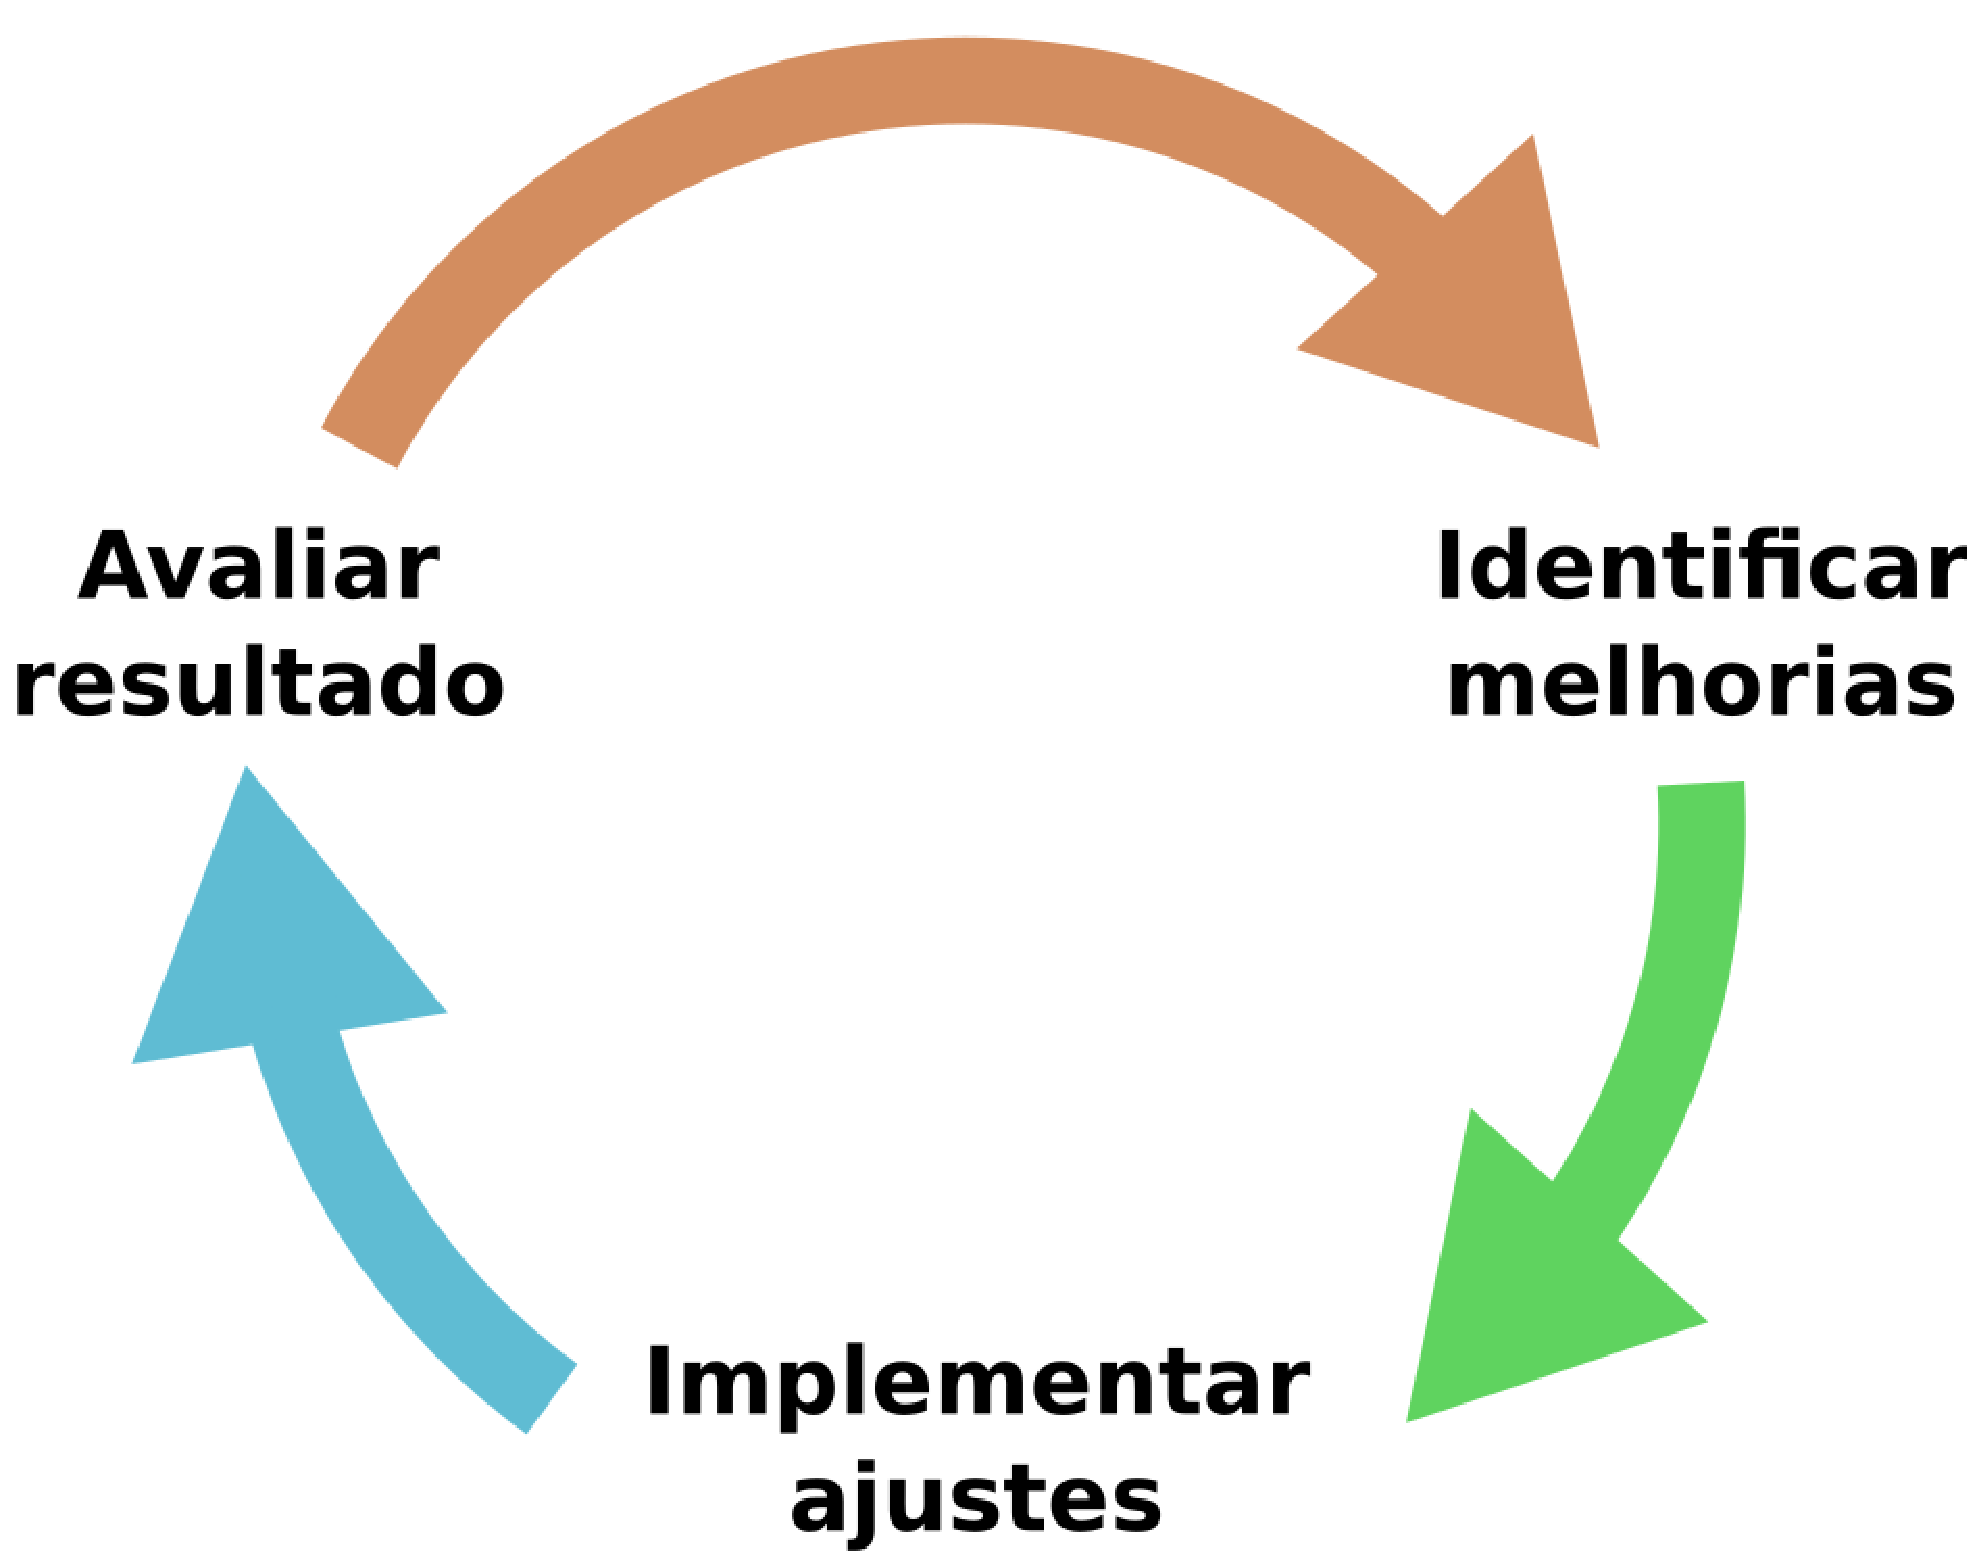
\includegraphics[scale=0.25]{metodologia}}%
			{Fonte: O autor (2025)}
			\label{fig:metodologia}
		\end{figure}
	\end{verbatim}

	Foi utilizado o pacote {\LaTeX} \cite{copyrightbox_package} para facilitar a adição das legendas das imagens que devem conter além da descrição, a informação da fonte utilizada.

	Tipicamente a informação da fonte costuma ser o dado do próprio autor, como visto do exemplo da  Fig~\ref{fig:metodologia}

	\begin{figure}[H]
		\centering
		\caption{Fluxo da metodologia itetariva utilizada no projeto.}
		\copyrightbox[b]{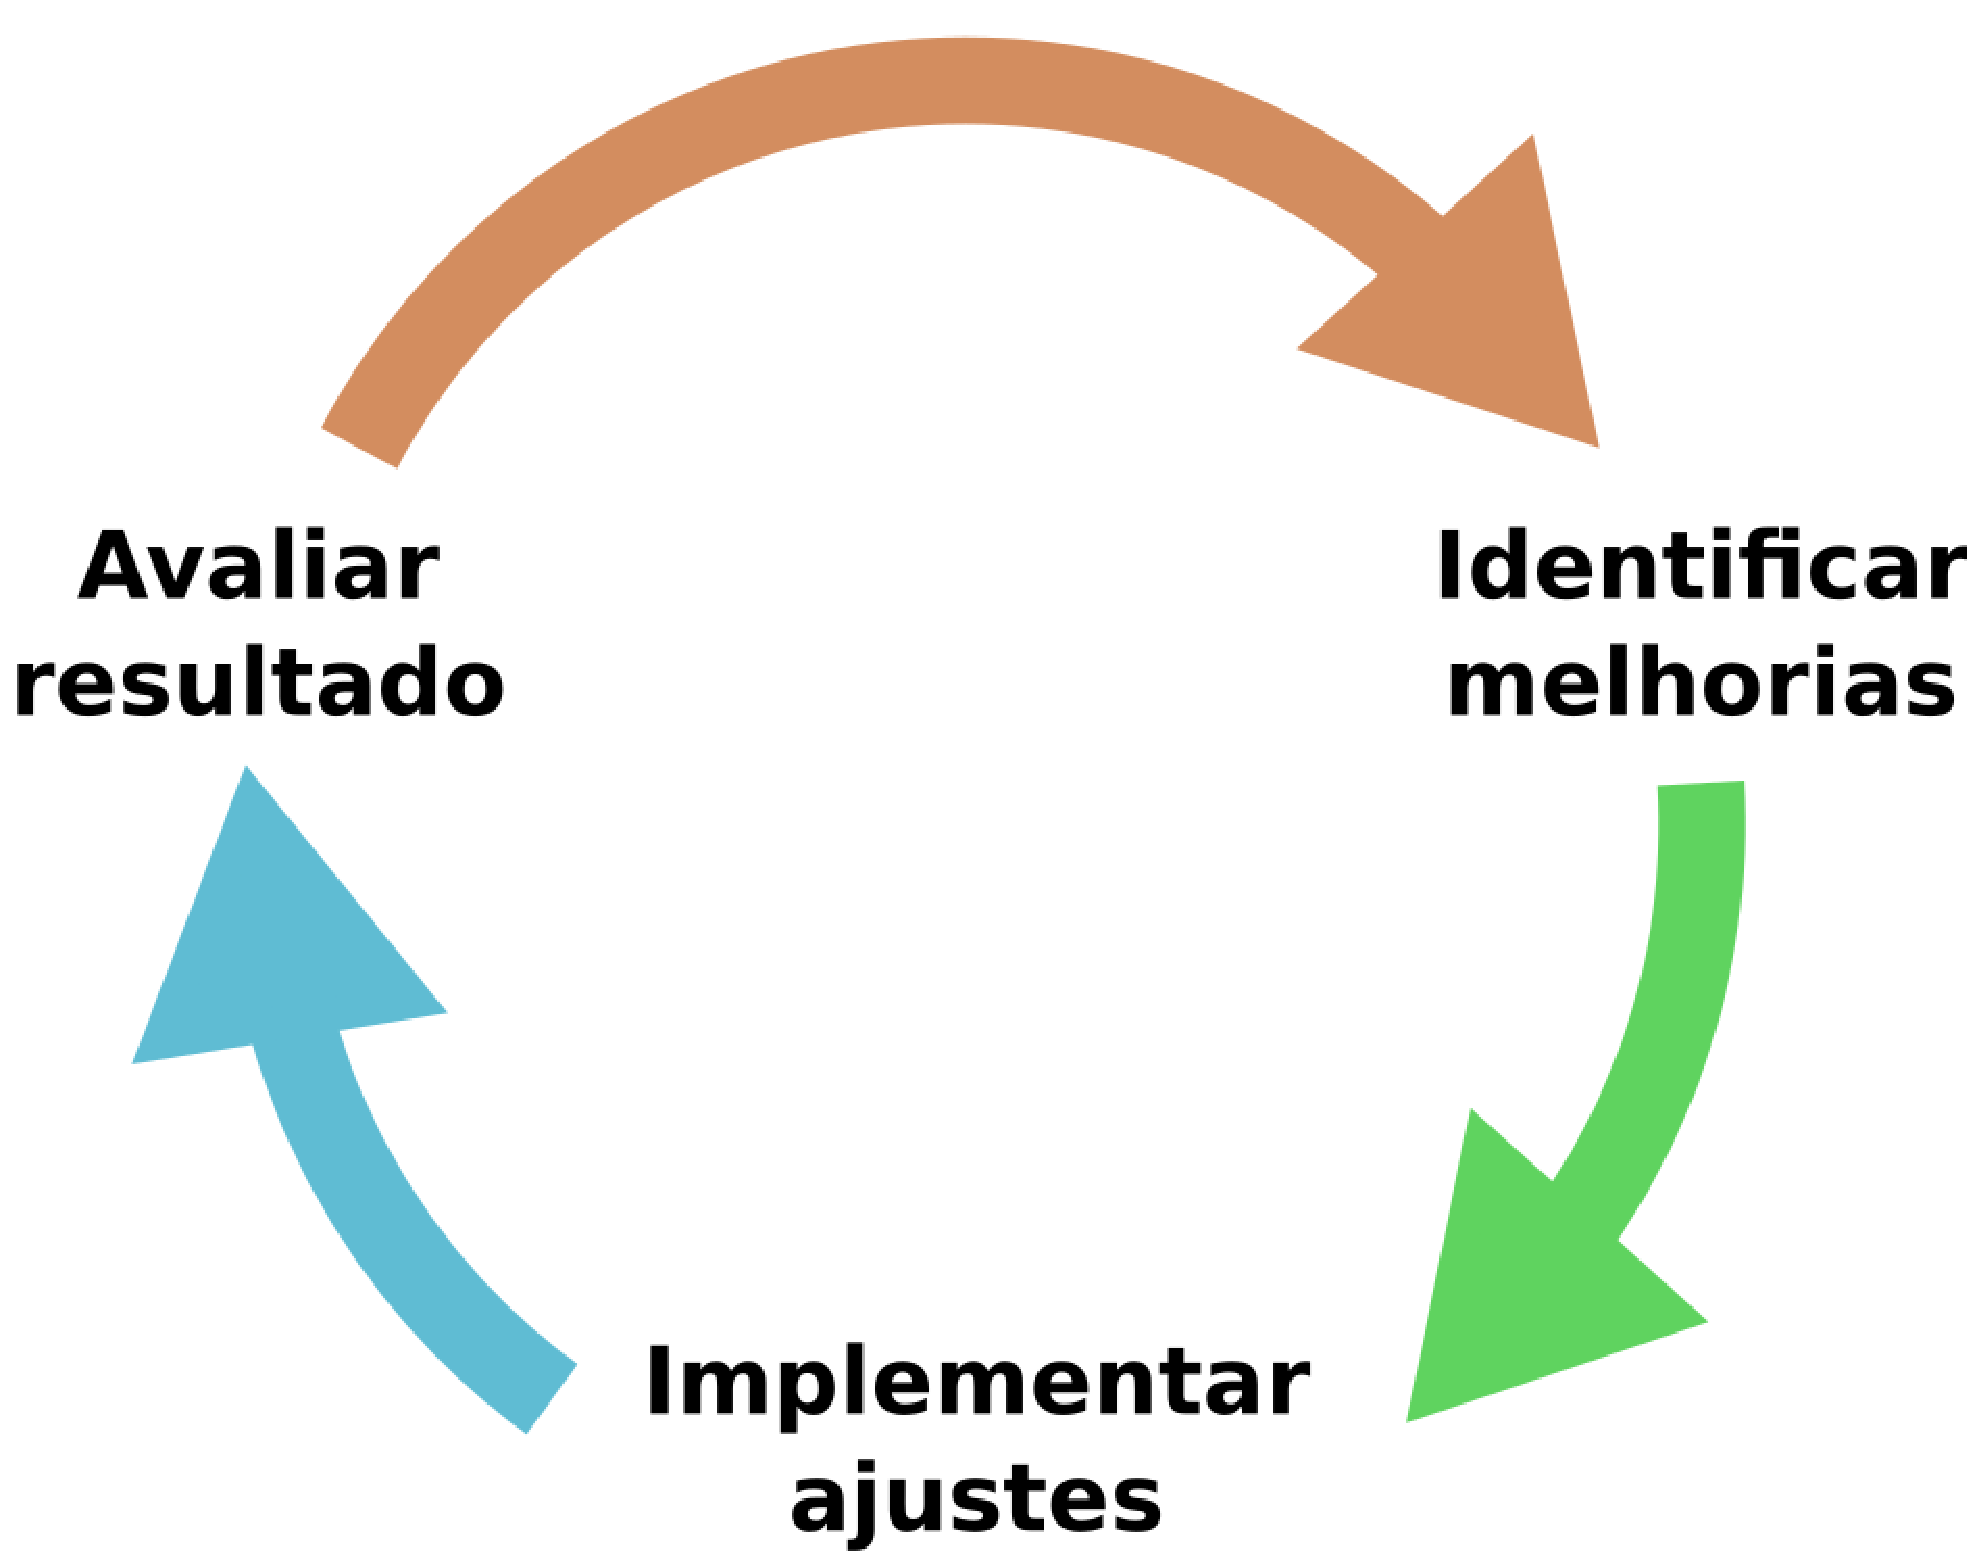
\includegraphics[scale=0.15]{metodologia}}%
		{Fonte: O autor (2025)}
		\label{fig:metodologia}
	\end{figure}

	Outra especificação da fonte comumente utilizada é uma citação convencional da fonte utilizada na imagem informando que a imagems utilizada foi exatamente a mesma, como demonstrado no exemplo da Fig~\ref{fig:mlapplication}.

	\begin{figure}[H]
		\centering
		\caption{Mapeamento das principais aplicações do aprendizado de máquina.}
		\copyrightbox[b]{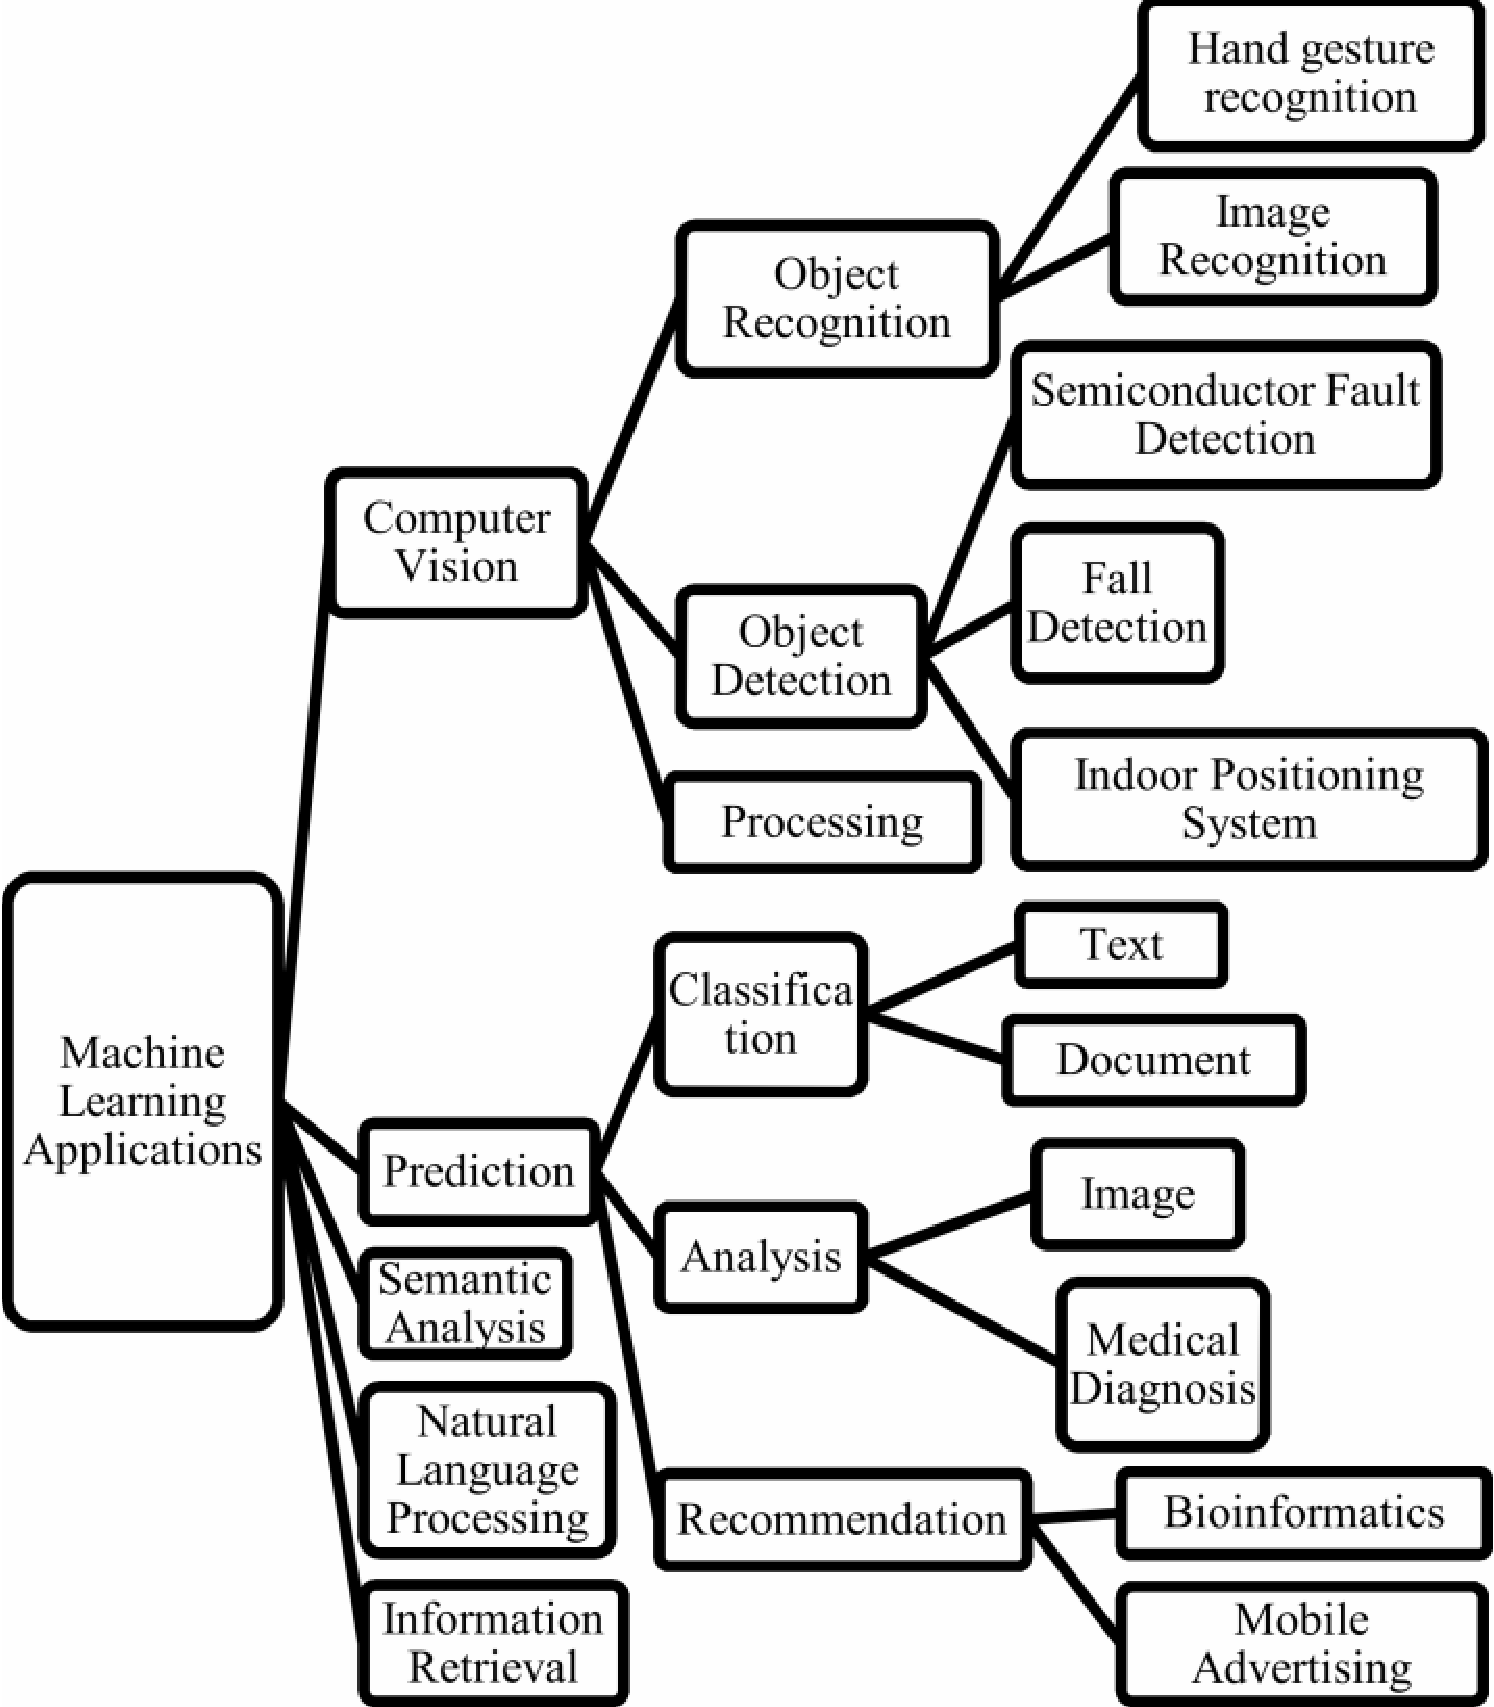
\includegraphics[width=0.7\linewidth]{mlapplications}}%
		{Fonte: Extraido de \cite{ApplicationMachineLearning}}
		\label{fig:mlapplication}
	\end{figure}

	Também é comun informar a referência, mas indicando que a imagem  foi adaptada para a sua utilização, como apresentada no exemplo da Fig~\ref{fig:fluxo_fsp}.

	\begin{figure}[H]
		\centering
		\caption{O fluxo básico de funcionamento da etapa de treinamento do FSP.}
		\copyrightbox[b]{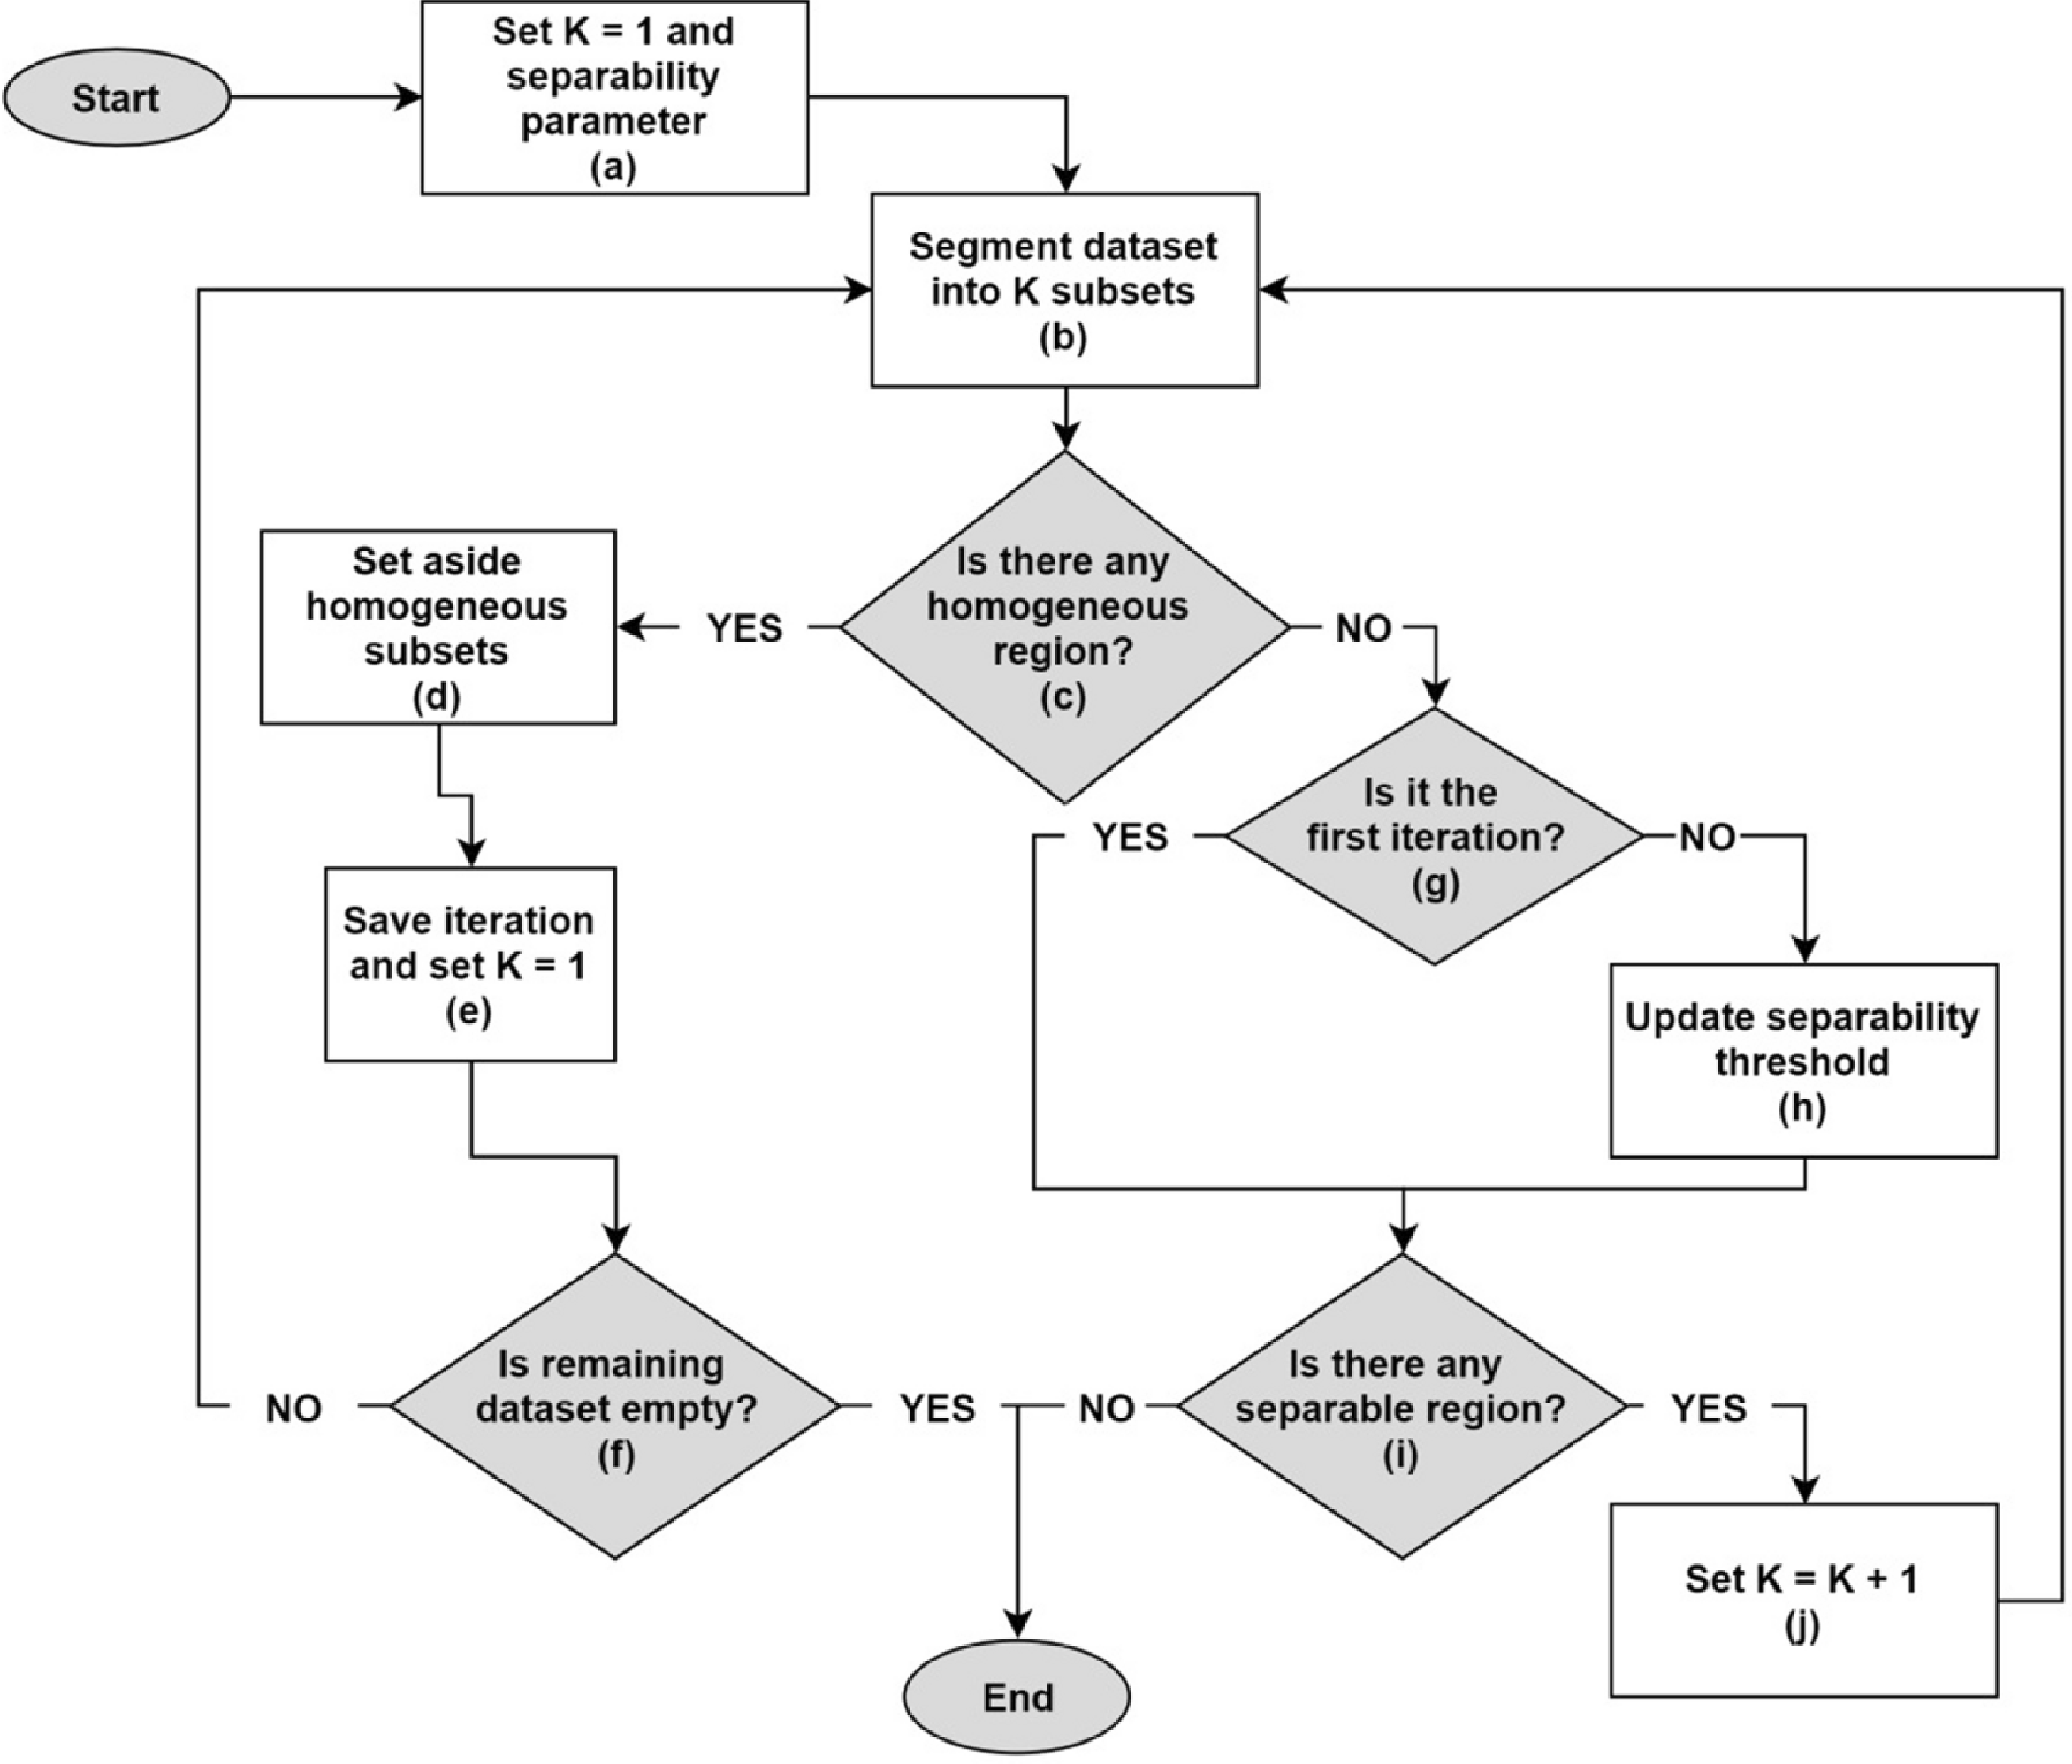
\includegraphics[scale=0.27]{fluxo_fsp}}%
		{Fonte: Adaptada de \cite{fsp-carolina}}
		\label{fig:fluxo_fsp}
	\end{figure}


	\item \MakeUppercase{Gráficos}

	As regras de formatação dos gráficos são similares as das imagens. É recomendado que durante a apresentação de um gráfico, as suas informações sejam claramente descritas de forma textual, para que qualquer pessoa mesmo sem a visualização do gráfico, consida entender do que se trata. As informações sobre as fontes com detalhamento da citação daquela referência ou indicação de criação do prórprio autor, também são as mesmas.

	O {\LaTeX} possui pacotes que permitem criar gráficos em tempo de compilação do documento. No Projeto Jacurutu, nenhum desse pacotes foram utilizados. A estratégia adaotada foi gerar imagens para os gráficos em outra ferramentas e salvar em formato PDF, em seguida incluir no documento como uma imagem. Essa estratégia é indicada como uma forma de melhorar a performance no processo de geração do documento final.

	Um exemplo de gráfico construído pelo autor pode ser visto na Fig~\ref{fig:tempoprocelectrical}.

	\begin{figure}[H]
		\centering
		\caption{Tempo de execução \textit{Electrical Fault Detection} X quantidade processos}
		\copyrightbox[b]{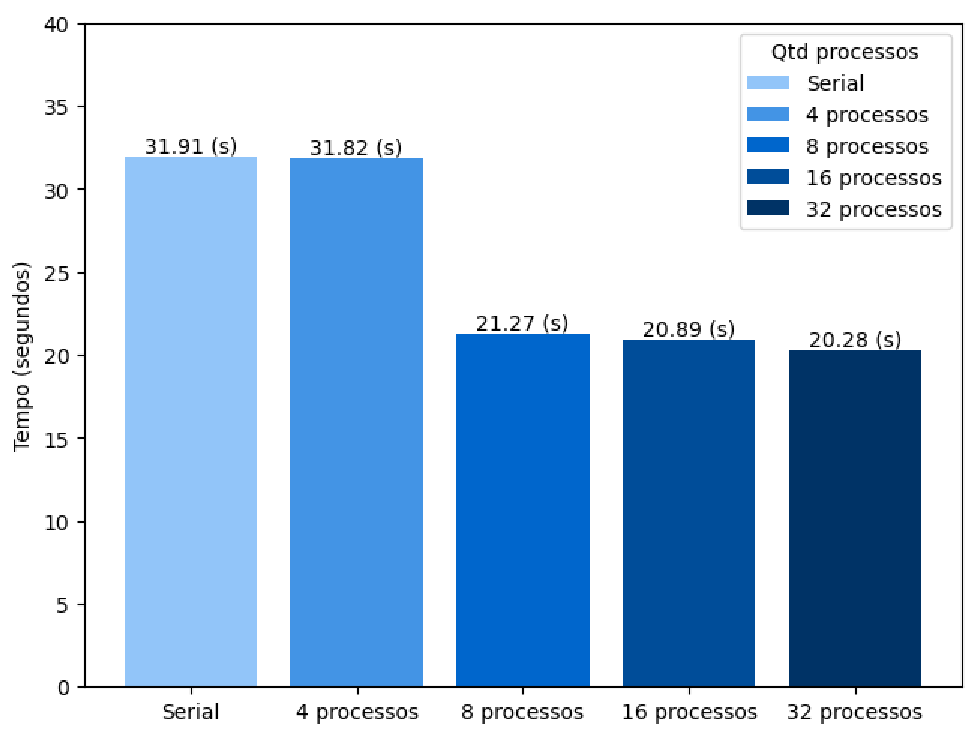
\includegraphics[width=0.9\linewidth]{electrical_process}}%
		{Fonte: O autor (2025)}
		\label{fig:tempoprocelectrical}
	\end{figure}

	\item \MakeUppercase{Tabelas}

	As regras de formatação das tabelas são similares as dos gráficos. É recomendado que durante a apresentação de uma tabelas, as suas informações sejam claramente descritas de forma textual, com explicação de todas as colunas, para que qualquer pessoa mesmo sem a visualização da mesma, consida entender do que se trata. As informações sobre as fontes com detalhamento da citação daquela referência ou indicação de criação do prórprio autor, também são as mesmas.

	A seguir um exemplo da criação de uma tabela simplificada e o seu resultado final, apresentado na Tabela~\ref{tab:tabelaexemplo1}.

	\begin{verbatim}
	\begin{table}
		\caption{Exemplo de tabela de uso genérico}
		\begin{center}
			\fontsize{10pt}{13pt}\selectfont
			\begin{tabular}{lcccc}
				\hline
				Bases & Observações & Features & Classe & Desbalanceamento\\
				& (used/total) & (used/total) & (used/total)  &           \\
				\hline
				Dataset1 & 150/150 &  4/4  & 3/3 & 1.00    \\
				Dataset3 & 208/208 & 60/60 & 2/2 & 1.14    \\
				Dataset3 & 214/214 & 9/10  & 6/7 & 8.44    \\
				\hline
				\multicolumn{5}{l}{Fonte: O autor (2025)}
			\end{tabular}
			\label{tab:tabelaexemplo1}
		\end{center}
	\end{table}
	\end{verbatim}
	
	\begin{table}[H]
		\caption{Exemplo de tabela de uso genérico}
		\begin{center}
			\fontsize{10pt}{13pt}\selectfont
			\begin{tabular}{lcccc}
				\hline
				Base de dados & Observações  &   Features   &   Classe  & Desbalanceamento\\
				& (used/total) & (used/total) & (used/total)  &                  \\
				\hline
				Dataset1 &   150/150    &     4/4      &     3/3       & 1.00    \\
				Dataset3 &   208/208    &    60/60     &     2/2       & 1.14    \\
				Dataset3 &   214/214    &     9/10     &     6/7       & 8.44    \\
				\hline
				\multicolumn{5}{l}{Fonte: O autor (2025)}
			\end{tabular}
			\label{tab:tabelaexemplo1}
		\end{center}
	\end{table}

	Também foi acicionado ao modelo um exemplo de tabela longa, usando o pacote longtable \cite{longtable_package}, que permite criar tabelas que se adaptam à quebra de página. Vale ressaltar que o alinhamento padrão desse pacote já é centralizado, e que ele já incrementa o contador das tabelas do documento. A seguir um exemplo de criação de uma tabela longa em \LaTeX, seguido da visualização do resultado da tabela, acessível na Tabela ~\ref{tab:long}
	
	\begin{verbatim}

		\begin{longtable}{|l|l|c|}
			\caption{Um exemplo de tabela longa.} \label{tab:long} \\
			
			\hline \multicolumn{1}{|c|}{\textbf{Coluna 1}} &
			 \multicolumn{1}{c|}{\textbf{Coluna 2}} &
			  \multicolumn{1}{c|}{\textbf{Coluna 3}} \\ \hline 
			\endfirsthead
			
			\multicolumn{3}{c}%
			{{\bfseries \tablename\ \thetable{} 
					-- continuação da página anterior}} \\
			\hline \multicolumn{1}{|c|}{\textbf{Coluna 1}} &
			 \multicolumn{1}{c|}{\textbf{Coluna 2}} &
			  \multicolumn{1}{c|}{\textbf{Coluna 3}} \\ \hline 
			\endhead
			
			\hline \multicolumn{3}{|r|}{{Continua na próxima 
					página}} \\ \hline
			\endfoot
			
			\hline \multicolumn{3}{l}{{Fonte: O autor (2025)}} \\
			\endlastfoot
			
			One & abcdef ghjijklmn & 123.456778 \\
			One & abcdef ghjijklmn & 123.456778 \\
			One & abcdef ghjijklmn & 123.456778 \\
			One & abcdef ghjijklmn & 123.456778 \\
			One & abcdef ghjijklmn & 123.456778 \\
			One & abcdef ghjijklmn & 123.456778 \\
			One & abcdef ghjijklmn & 123.456778 \\
			One & abcdef ghjijklmn & 123.456778 \\
			One & abcdef ghjijklmn & 123.456778 \\
			One & abcdef ghjijklmn & 123.456778 \\
			One & abcdef ghjijklmn & 123.456778 \\
			One & abcdef ghjijklmn & 123.456778 \\
			One & abcdef ghjijklmn & 123.456778 \\
			One & abcdef ghjijklmn & 123.456778 \\
			One & abcdef ghjijklmn & 123.456778 \\
			One & abcdef ghjijklmn & 123.456778 \\
			One & abcdef ghjijklmn & 123.456778 \\
			One & abcdef ghjijklmn & 123.456778 \\
			One & abcdef ghjijklmn & 123.456778 \\
			One & abcdef ghjijklmn & 123.456778 \\
			One & abcdef ghjijklmn & 123.456778 \\
			One & abcdef ghjijklmn & 123.456778 \\
			One & abcdef ghjijklmn & 123.456778 \\
			One & abcdef ghjijklmn & 123.456778 \\
			One & abcdef ghjijklmn & 123.456778 \\
			One & abcdef ghjijklmn & 123.456778 \\
			One & abcdef ghjijklmn & 123.456778 \\
			One & abcdef ghjijklmn & 123.456778 \\
			One & abcdef ghjijklmn & 123.456778 \\
			One & abcdef ghjijklmn & 123.456778 \\
			One & abcdef ghjijklmn & 123.456778 \\
			One & abcdef ghjijklmn & 123.456778 \\
			One & abcdef ghjijklmn & 123.456778 \\
			One & abcdef ghjijklmn & 123.456778 \\
			One & abcdef ghjijklmn & 123.456778 \\
			One & abcdef ghjijklmn & 123.456778 \\
			One & abcdef ghjijklmn & 123.456778 \\
			One & abcdef ghjijklmn & 123.456778 \\
			One & abcdef ghjijklmn & 123.456778 \\
			One & abcdef ghjijklmn & 123.456778 \\
			One & abcdef ghjijklmn & 123.456778 \\
			One & abcdef ghjijklmn & 123.456778 \\
			One & abcdef ghjijklmn & 123.456778 \\
			One & abcdef ghjijklmn & 123.456778 \\
			One & abcdef ghjijklmn & 123.456778 \\
			One & abcdef ghjijklmn & 123.456778 \\
			One & abcdef ghjijklmn & 123.456778 \\
			One & abcdef ghjijklmn & 123.456778 \\
			One & abcdef ghjijklmn & 123.456778 \\
			One & abcdef ghjijklmn & 123.456778 \\
			One & abcdef ghjijklmn & 123.456778 \\
			One & abcdef ghjijklmn & 123.456778 \\
			One & abcdef ghjijklmn & 123.456778 \\
			One & abcdef ghjijklmn & 123.456778 \\
			One & abcdef ghjijklmn & 123.456778 \\
			One & abcdef ghjijklmn & 123.456778 \\
			One & abcdef ghjijklmn & 123.456778 \\
			One & abcdef ghjijklmn & 123.456778 \\
			One & abcdef ghjijklmn & 123.456778 \\
			One & abcdef ghjijklmn & 123.456778 \\
			One & abcdef ghjijklmn & 123.456778 \\
			One & abcdef ghjijklmn & 123.456778 \\
			One & abcdef ghjijklmn & 123.456778 \\
			One & abcdef ghjijklmn & 123.456778 \\
			One & abcdef ghjijklmn & 123.456778 \\
			One & abcdef ghjijklmn & 123.456778 \\
			One & abcdef ghjijklmn & 123.456778 \\
			One & abcdef ghjijklmn & 123.456778 \\
			One & abcdef ghjijklmn & 123.456778 \\
			One & abcdef ghjijklmn & 123.456778 \\
			One & abcdef ghjijklmn & 123.456778 \\
			One & abcdef ghjijklmn & 123.456778 \\
			One & abcdef ghjijklmn & 123.456778 \\
			One & abcdef ghjijklmn & 123.456778 \\
			One & abcdef ghjijklmn & 123.456778 \\
			One & abcdef ghjijklmn & 123.456778 \\
			One & abcdef ghjijklmn & 123.456778 \\
			One & abcdef ghjijklmn & 123.456778 \\
			One & abcdef ghjijklmn & 123.456778 \\
			One & abcdef ghjijklmn & 123.456778 \\
		\end{longtable}

	\end{verbatim}	
	
\begin{longtable}{|l|l|c|}
	\caption{Um exemplo de tabela longa.} \label{tab:long} \\
	
	\hline \multicolumn{1}{|c|}{\textbf{Coluna 1}} & \multicolumn{1}{c|}{\textbf{Coluna 2}} & \multicolumn{1}{c|}{\textbf{Coluna 3}} \\ \hline 
	\endfirsthead
	
	\multicolumn{3}{c}%
	{{\bfseries \tablename\ \thetable{} -- continuação da página anterior}} \\
	\hline \multicolumn{1}{|c|}{\textbf{Coluna 1}} & \multicolumn{1}{c|}{\textbf{Coluna 2}} & \multicolumn{1}{c|}{\textbf{Coluna 3}} \\ \hline 
	\endhead
	
	\hline \multicolumn{3}{|r|}{{Continua na próxima página}} \\ \hline
	\endfoot
	
	\hline \multicolumn{3}{l}{{Fonte: O autor (2025)}} \\
	\endlastfoot
	
	One & abcdef ghjijklmn & 123.456778 \\
	One & abcdef ghjijklmn & 123.456778 \\
	One & abcdef ghjijklmn & 123.456778 \\
	One & abcdef ghjijklmn & 123.456778 \\
	One & abcdef ghjijklmn & 123.456778 \\
	One & abcdef ghjijklmn & 123.456778 \\
	One & abcdef ghjijklmn & 123.456778 \\
	One & abcdef ghjijklmn & 123.456778 \\
	One & abcdef ghjijklmn & 123.456778 \\
	One & abcdef ghjijklmn & 123.456778 \\
	One & abcdef ghjijklmn & 123.456778 \\
	One & abcdef ghjijklmn & 123.456778 \\
	One & abcdef ghjijklmn & 123.456778 \\
	One & abcdef ghjijklmn & 123.456778 \\
	One & abcdef ghjijklmn & 123.456778 \\
	One & abcdef ghjijklmn & 123.456778 \\
	One & abcdef ghjijklmn & 123.456778 \\
	One & abcdef ghjijklmn & 123.456778 \\
	One & abcdef ghjijklmn & 123.456778 \\
	One & abcdef ghjijklmn & 123.456778 \\
	One & abcdef ghjijklmn & 123.456778 \\
	One & abcdef ghjijklmn & 123.456778 \\
	One & abcdef ghjijklmn & 123.456778 \\
	One & abcdef ghjijklmn & 123.456778 \\
	One & abcdef ghjijklmn & 123.456778 \\
	One & abcdef ghjijklmn & 123.456778 \\
	One & abcdef ghjijklmn & 123.456778 \\
	One & abcdef ghjijklmn & 123.456778 \\
	One & abcdef ghjijklmn & 123.456778 \\
	One & abcdef ghjijklmn & 123.456778 \\
	One & abcdef ghjijklmn & 123.456778 \\
	One & abcdef ghjijklmn & 123.456778 \\
	One & abcdef ghjijklmn & 123.456778 \\
	One & abcdef ghjijklmn & 123.456778 \\
	One & abcdef ghjijklmn & 123.456778 \\
	One & abcdef ghjijklmn & 123.456778 \\
	One & abcdef ghjijklmn & 123.456778 \\
	One & abcdef ghjijklmn & 123.456778 \\
	One & abcdef ghjijklmn & 123.456778 \\
	One & abcdef ghjijklmn & 123.456778 \\
	One & abcdef ghjijklmn & 123.456778 \\
	One & abcdef ghjijklmn & 123.456778 \\
	One & abcdef ghjijklmn & 123.456778 \\
	One & abcdef ghjijklmn & 123.456778 \\
	One & abcdef ghjijklmn & 123.456778 \\
	One & abcdef ghjijklmn & 123.456778 \\
	One & abcdef ghjijklmn & 123.456778 \\
	One & abcdef ghjijklmn & 123.456778 \\
	One & abcdef ghjijklmn & 123.456778 \\
	One & abcdef ghjijklmn & 123.456778 \\
	One & abcdef ghjijklmn & 123.456778 \\
	One & abcdef ghjijklmn & 123.456778 \\
	One & abcdef ghjijklmn & 123.456778 \\
	One & abcdef ghjijklmn & 123.456778 \\
	One & abcdef ghjijklmn & 123.456778 \\
	One & abcdef ghjijklmn & 123.456778 \\
	One & abcdef ghjijklmn & 123.456778 \\
	One & abcdef ghjijklmn & 123.456778 \\
	One & abcdef ghjijklmn & 123.456778 \\
	One & abcdef ghjijklmn & 123.456778 \\
	One & abcdef ghjijklmn & 123.456778 \\
	One & abcdef ghjijklmn & 123.456778 \\
	One & abcdef ghjijklmn & 123.456778 \\
	One & abcdef ghjijklmn & 123.456778 \\
	One & abcdef ghjijklmn & 123.456778 \\
	One & abcdef ghjijklmn & 123.456778 \\
	One & abcdef ghjijklmn & 123.456778 \\
	One & abcdef ghjijklmn & 123.456778 \\
	One & abcdef ghjijklmn & 123.456778 \\
	One & abcdef ghjijklmn & 123.456778 \\
	One & abcdef ghjijklmn & 123.456778 \\
	One & abcdef ghjijklmn & 123.456778 \\
	One & abcdef ghjijklmn & 123.456778 \\
	One & abcdef ghjijklmn & 123.456778 \\
	One & abcdef ghjijklmn & 123.456778 \\
	One & abcdef ghjijklmn & 123.456778 \\
	One & abcdef ghjijklmn & 123.456778 \\
	One & abcdef ghjijklmn & 123.456778 \\
	One & abcdef ghjijklmn & 123.456778 \\
	One & abcdef ghjijklmn & 123.456778 \\
\end{longtable}
	
	\item \MakeUppercase{Listas}

	As listas utilizadas no modelo (se numeração) seguem a configuração nativa do próprio latex, e para utilizá-las, não é necessário adicionar nenhum pacote extra.

	Um exemplo de lista pode ser criada utilizando os comandos \verb|\begin{itemize}| e \verb|\item|, como demostrado a seguir:

	\begin{verbatim}
		\begin{itemize}
			\item Primeiro item da lista não numerada.
			\item Segundo item
			\item Terceiro item.
		\end{itemize}
	\end{verbatim}

	Tendo como uma lista como a apresentada abaixo:

	\begin{itemize}
		\item Primeiro item da lista não numerada.
		\item Segundo item
	\end{itemize}

	Também é possível criar sub hierarquia de listas, simplemente criando novos blocos do comando \verb|\begin{itemize}|, dentro de um já existente.

	\begin{verbatim}
	\begin{itemize}
		\item Primeiro item da lista não numerada.
		\item Segundo item, que pode ter um subitem:
		\begin{itemize}
			\item Subitem não numerado.
			\item Outro subitem.
		\end{itemize}
		\item Terceiro item.
	\end{itemize}
	\end{verbatim}

	O resultado final é apresentado a seguir:

	\begin{itemize}
		\item Primeiro item da lista não numerada.
		\item Segundo item, que pode ter um subitem:
		\begin{itemize}
			\item Subitem não numerado.
			\item Outro subitem.
		\end{itemize}
		\item Terceiro item.
	\end{itemize}

	\item \MakeUppercase{Listas Enumeradas}

	As listas enumeradas possuem um comportamento parecido com os das listas convencionais. No seu comportamento mais simples, também não é necessário nenhum pacote extra, para a sua utilização.

	O exemplo a seguir, demonstra como construir uma lista enumerada de forma simplificada:

	\begin{verbatim}
		\begin{enumerate}
			\item Primeiro item da lista.
			\item Segundo item da lista.
			\begin{enumerate}
				\item Subitem do segundo item.
				\item Outro subitem.
			\end{enumerate}
			\item Terceiro item.
		\end{enumerate}
	\end{verbatim}

	É possível observar na sequência, o resultado dessa listagem:

	\begin{enumerate}
		\item Primeiro item da lista.
		\item Segundo item da lista.
		\begin{enumerate}
			\item Subitem do segundo item.
			\item Outro subitem.
		\end{enumerate}
		\item Terceiro item.
	\end{enumerate}

	O modelo configura por padrão um pacote chamado enumitem \cite{enumitem_package}, onde é possível configurar qual o tipo do elemento de contagem que será apresentado em cada nível (como arabiço, romano ou alfabetico), bem como definir prefixos, sufixo e retomar uma contagem de um ponto prévio em outro local do texto, o que pode permitir formatações interessantes durante uma listagem.

	No exemplo a seguir, foi alterado os tipos dos algarítimos utilizados na contagem, alem de ter sido modificado o padrão da numeração para apenas um parêntese após a numeração:

	\begin{verbatim}
		\begin{enumerate}[label=\arabic*)] % Números romanos em parênteses
			\item Item em arábico.
			\item Outro item.
			\begin{enumerate}[label=\alph*)]
				\item Subitem do segundo item.
				\item Outro subitem.
			\end{enumerate}
			\item Terceiro item.
		\end{enumerate}
	\end{verbatim}

	O resultado pode ser visualizado a seguir:

	\begin{enumerate}[label=\arabic*)] % Números romanos em parênteses
		\item Item em arábico.
		\item Outro item.
		\begin{enumerate}[label=\alph*)]
			\item Subitem do segundo item.
			\item Outro subitem.
		\end{enumerate}
		\item Terceiro item.
	\end{enumerate}

	É possível com essa abordagem por exemplo, utilizar uma lista enumerada para apresentar ums listagem específica do seu trabalho, como por exemplo a lista de questões de pesquisa que o seu trabalho tenat responder:

	\begin{verbatim}
		\begin{enumerate}[label=\textbf{QP\arabic* -}]
			\item A dinâmica da execução do método de classificação FSP...?
			\item Quais estratégias de paralelização trazem melhores...?
			\item É possível realizar esse processo de paralelização ...?
		\end{enumerate}
	\end{verbatim}

	O que seria apresentado da seguinte forma:

	\begin{enumerate}[label=\textbf{QP\arabic* -}]
		\item A dinâmica da execução do método de classificação FSP...?
		\item Quais estratégias de paralelização trazem melhores...?
		\item É possível realizar esse processo de paralelização ...?
	\end{enumerate}
	
	O Apêndice C também apresenta um formulário, onde uma lista enumerada foi utilizada para realizar a formatação das suas questões.

	\item \MakeUppercase{Equações e fórmulas}

	As definições de equações e fórmulas são um recurso nativo do {\LaTeX} e com isso nenhum pacote extra é necessário para ter acesso a esse tipo de recurso. Entretanto o pacote amsmath \cite{amsmath_package} foi adicionado ao modelo para permitir criar referências internas entre as equações e formulas e suas descrições no texto através do comando \verb|\eqref{label}|.

	Também é comum que ao inserir uma equaçaão, sua descrição também seja a mais detalhada possível, possibilitando um possível entendimento mesmo apenas com a leitura da descrição.

	A utilização de equações e fórmulas não necessitam por padrão de uma listagem que contemple todas as equações e formulas utilizadas no trabalho, como acontecem com as figiras e tabelas.

	O seguinte exemplo apresenta a criação de uma equação com uma descrição detalhada e uma referencia usando o comando \verb|\eqref{label}|.

	\begin{verbatim}
		Essa métrica é estabelecida pela equação
		~\eqref{eq:diferenca_percentual}, onde \(DP\)
		é a Diferença Percentual, \(T_p\) é o Tempo em Paralelo
		e \(T_s\) é o Tempo Serial.

		\begin{equation}
			DP = (T_p - T_s) / T_s * 100
			\label{eq:diferenca_percentual}
		\end{equation}
	\end{verbatim}


	O reultado é apresentado a seguir:

	Essa métrica é estabelecida pela equação~\eqref{eq:diferenca_percentual}, onde \(DP\) é a Diferença Percentual, \(T_p\) é o Tempo em Paralelo e \(T_s\) é o Tempo Serial.

	\begin{equation}
		DP = (T_p - T_s) / T_s * 100
		\label{eq:diferenca_percentual}
	\end{equation}

	\item \MakeUppercase{Links Externos (URL)}

	Como o modelo já configura o pacote {\LaTeX} URL \cite{url_package}, caso deseje informar um link externo no seu texto (URL), basta utilizar o comando \verb|\url{link}|. Como o podelo também já configura o pacote {\LaTeX} Hyperref \cite{hyperref_package}, esse link será apresentado em formato de link acessível no próprio documento -- ao passar o mouse sobre o link --, como podemos ver no exemplo que segue:

	\begin{verbatim}
	Também foi criado um DOI para identificar univocamente essa
	implementação, e pode ser acessada em:
	\url{https://doi.org/10.5281/zenodo.16969842}.
	\end{verbatim}

	Segue o resultado da criação da URL:

	Também foi criado um DOI para identificar univocamente essa implementação, e pode ser acessada em: \url{https://doi.org/10.5281/zenodo.16969842}.


\end{enumerate}

	%Exemplo de apêndice (desenvolvido pelo autor) (elemento opcional)
	\input{3-pos-textuais/apendice-b}

	%Exemplo de apêndice (desenvolvido pelo autor) (elemento opcional)
	\input{3-pos-textuais/apendice-c}

	%Exemplo de anexo (não foi desenvolvido pelo autor) (elemento opcional)
	\input{3-pos-textuais/anexo-a}

	%Índice remissívo (elemento opcional)
	\input{3-pos-textuais/indice}

\end{document}